\documentclass[reqno]{amsart}
\usepackage[utf8]{inputenc}

\usepackage{sky}
\usepackage{graphicx}
\usepackage{color}
\usepackage{caption}
\usepackage{subcaption}


\setcounter{tocdepth}{1}

\newcommand{\epe}{\mrm{EPE}}
\newcommand{\area}{\mrm{area}}
\newcommand{\excited}{\Gamma}
\newcommand{\Wg}{\mrm{Wg}}
\newcommand{\symgrp}{\mrm{S}}
\newcommand{\bP}{\mbf{P}}
\newcommand{\neighbors}{\ms{N}}
\newcommand{\map}{\mathfrak{m}}
\newcommand{\roote}{\mathfrak{r}}
\newcommand{\CF}{\mrm{CF}}
\newcommand{\tail}{\tau}
\newcommand{\modarea}{\underbar{area}}
\newcommand{\vertiii}[1]{{\left\vert\kern-0.25ex\left\vert\kern-0.25ex\left\vert #1 
\right\vert\kern-0.25ex\right\vert\kern-0.25ex\right\vert}}
\newcommand{\sym}{S_{\mathrm{YM}}}



\newcommand{\ron}[1]{\textcolor{green}{[Ron: #1]}}
\newcommand{\sky}[1]{\textcolor{blue}{[Sky: #1]}}
\newcommand{\scott}[1]{\textcolor{purple}{[Scott: #1]}}


\title{Perimeter law lower bound for center-neutral Yang--Mills theories}

% \author{Sky Cao}
% \address{Department of Mathematics, Massachusetts Institute of Technology, Cambridge, MA 02139}
% \email{skycao@mit.edu}

\author{Ron Nissim}
\address{Ron Nissim, Department of Mathematics, Massachusetts Institute of Technology, Cambridge, MA 02139}
\email{rnissim@mit.edu}

\date{}

\begin{document}

\begin{abstract}
    We show that for pure lattice Yang--Mills theories in dimension $d\geq 3$, any Wilson loop observable associated with a coordinate rectangle and a center-neutral representation satisfies a perimeter law lower bound. This result holds at weak coupling, which is most relevant to the continuum theory, under the assumption that the model has a translation-invariant infinite-volume limit.
\end{abstract}

\maketitle

\tableofcontents

\section{Introduction}

Euclidean quantum Yang--Mills theory is the mathematical framework for the standard model of particle physics. In order to initiate a rigorous mathematical treatment of the subject, \cite{Wilson1974} introduced a lattice version of the model referred to as lattice Yang--Mills theory. Wilson was additionally motivated by laying out a mathematical criterion for quark confinement: the physical phenomenon that quarks are not observed in isolation. His condition for quark confinement requires a faster than perimeter rate of exponential decay of the Wilson loop expectation associated to rectangular loops. 

Our main result, Theorem \ref{thm:Main-theorem}, states that Wilson's criterion is not satisfied whenever Wilson loop observables are `insensitive' to the center of the gauge group of the model by providing an exponential in perimeter lower bound on rectangular Wilson loop expectations. The notion of being `insensitive' to the center of the gauge group will be made precise in Definition \ref{def:center-neutral}.

\subsection{Relation to Prior Literature}

In the strong coupling regime of lattice Yang--Mills theories, a strong form of Wilson's confinement criterion known as area law, requiring exponential in area decay of the rectangular Wilson loop expectation, is known to hold whenever the center acts on the Wilson representation by a nontrivial character \cite{osterwalderseiler1978,seiler1982gauge}. The proof idea of these works is to perform a strong coupling cluster expansion for the Wilson loop expectation, and use the symmetry granted by sensitivity to the center to argue that any nonzero contribution to the cluster expansion requires the loop to be connected to a cluster at least the size of the area of the loop. More recent work improves the regime of parameters for which area law holds, but it still crucially requires sensitivity to the center of the gauge group \cite{CNS2025a,CNS2025b}. 


In the other direction, in \cite{GlimmJaffeNonConfinement,seiler1982gauge} the authors argue that under center `insensitivity' assumptions similar to Definition \ref{def:center-neutral}, the strong coupling cluster expansion for a Wilson loop expectation contains nonzero contributions from clusters of size proportional to the perimeter of the loop when the space--time dimension $d \geq 3$, and thus the Wilson loop expectation should exhibit a perimeter law lower bound. This argument is difficult to make rigorous because contributions to the cluster expansion are signed and it is not obvious that the contributions to the cluster expansion do not all cancel out.

In a recent article \cite{nissim2026deconfinementmathrmso3latticeyangmills}, the author was able to turn the cluster expansion argument into a rigorous proof that Wilson's criterion is not satisfied for $G =\mrm{SO}(3)$ with the defining Wilson representation in a strong coupling regime. This argument required additional inputs from complex analysis and reflection positivity and the analysis of the cluster expansion is specific to $\mathrm{SO}(3)$. The precise statement does not guarantee a perimeter law lower bound and excludes a Lebesgue measure $0$ set of $\beta$ values in the strong coupling interval. 

This work proves a perimeter law lower bound, applies to a much more general setting with any gauge group and Wilson representation satisfying a center neutrality assumption, and also holds at weak coupling under an assumption regarding the existence of a translation-invariant infinite-volume measure.

The approach is also quite different from that of \cite{nissim2026deconfinementmathrmso3latticeyangmills}, and does not directly involve any cluster expansion. Inspiration for this argument can be traced to two ideas from the physics literature. The first idea is that in cases when the gauge group and Wilson representation satisfy a center neutrality condition, it is possible to use the pure gauge field on edges to construct a vector-valued field on vertices which transforms like a Higgs field under gauge transformations. Since the pure gauge field describes gluons, and this Higgs-like field behaves like a massive particle made from gluons, physicists refer to it as a `gluelump.' To the author's knowledge, the construction first appeared in \cite{Michael1985AdjointSources} for the case of gauge group $\mathrm{SU}(2)$ with adjoint Wilson representation, and has been extensively studied since, primarily in the numerical lattice gauge theory literature (a very incomplete list includes \cite{JoryszMichael1988FieldConfigurations,PhilipsenWittig1999AdjointStringBreaking,PepeWiese2009StringDecay}). In this work we generalize the construction to all groups with center-neutral representations and highlight the general, but elementary, representation theory behind the construction.

The second idea is that through iterated reflection positivity Cauchy--Schwarz applied to gauge-invariant Wilson line observables, a perimeter law lower bound can be shown for the lattice Yang--Mills--Higgs model \cite{EvertzEtAl1987Perimeter}. Feeding the Higgs-like gluelump field into this argument completes the proof. One key place where our proof diverges from the treatment of \cite{EvertzEtAl1987Perimeter} is the additional argument to ensure the one-edge `Wilson line' is bounded below in the infinite volume setting, even at weak coupling in Lemma \ref{lm:one-edge-positivity}.


We now state the precise main result along with the definitions underlying the model.

\subsection{Main Result}

First we recall some definitions and notation relating to the lattice Yang--Mills model. Let $G$ be a compact Lie group. For integers $L\geq1$, set $\Lambda_L^i = ([-L,L]^{i-1}\times[-L,L+1] \times [-L,L]^{d-i})\cap\Z^d$. Write $e_i$ for the $i$th coordinate unit vector.  Let $E_{\Lambda}^+$ (resp. $E_\Lambda$) be the collection of positively oriented (resp. oriented) edges in $\Lambda$. Similarly, let $\mc{P}_{\Lambda}^+$ (resp. $\mc{P}_{\Lambda}$) denote the set of positively oriented (resp. oriented) plaquettes in $\Lambda$. For oriented edges $e \in E_\Lambda$, we denote by $e^{-1}$ the oppositely oriented version of $e$. Similarly, for oriented plaquettes $p \in \mc{P}_\Lambda$, we denote by $p^{-1}$ the oppositely oriented version of $p$.

\begin{definition}[Lattice gauge configuration]\label{def:gauge-configuration}
A lattice gauge configuration $Q$ is a function $Q : E_\Lambda^+ \ra G$. We always implicitly extend $Q : E_\Lambda \ra G$ to oriented edges, by imposing that $Q_{e^{-1}} := Q_e^{-1}$ for all $e \in E_\Lambda^+$.
\end{definition}

\begin{remark}
    We can, and usually will, equivalently identify the set of gauge configurations with $G^{E_{\Lambda}^+}$.
\end{remark}

\begin{definition}[Plaquette variable]
Given a lattice gauge configuration $Q : E_\Lambda^+ \ra G$ and an oriented plaquette $p = e_1 e_2 e_3 e_4$, we define the plaquette variable (abusing notation)
\begin{equs}
Q_p := Q_{e_1} Q_{e_2} Q_{e_3} Q_{e_4}.
\end{equs}
\end{definition}

Next, we define the lattice Yang--Mills measure. In order to do so we specify a faithful continuous unitary representation $\sigma: G \to \mrm{U}(V)$ where $V$ is a nonzero finite-dimensional complex Hilbert space and $\mrm{U}(V)$ denotes the set of unitary operators on $V$. Recall that faithful just means that $\sigma$ is injective as a function.

\begin{definition}[Lattice Yang--Mills]\label{def:lattice-ym}
The \textit{lattice Yang--Mills measure} with Wilson action specified by the faithful continuous (finite-dimensional) unitary representation $\sigma$, gauge group $G$, and inverse coupling $\beta>0$ on a finite subgraph $\Lambda \subset \Z^d$ is the measure on $G^{E_{\Lambda}^+}$ with density
\begin{equs}
    d\mu_{G,\sigma,\Lambda, \beta}(Q) \, \, \propto \, \, \exp(S_{G,\sigma,\Lambda, \beta}(Q)) dQ,
\end{equs}
where the action is given by
\begin{equs}
    S_{G,\sigma,\Lambda, \beta}(Q):=\beta\sum_{p \in \mc{P}_{\Lambda}} \chi_{\sigma}(Q_p)
    =2\beta\sum_{p\in\mc{P}_{\Lambda}^+}\mrm{Re}\,\chi_\sigma(Q_p),
\end{equs}
with $\chi_{\sigma}(Q)$ the character defined by $\chi_{\sigma}(Q):= \mrm{Tr} \sigma(Q)$ and $dQ = \prod_{e \in E_\Lambda^+} dQ_e$, where each $dQ_e$ is an independent copy of Haar measure on $G$. Finally, the partition function is
\begin{equs}
Z_{G,\sigma,\Lambda, \beta} :=\int_{G^{E_{\Lambda}^+}} \exp(S_{G,\sigma,\Lambda, \beta}(Q)) dQ.
\end{equs}
Since $G,\sigma,\beta$ are fixed throughout the argument, we will often use the notation $\langle \cdot \rangle_{\Lambda}$ to denote the expectation with respect to the probability measure $\mu_{G,\sigma,\Lambda, \beta}$.
\end{definition}

Next we define the main observable of interest throughout the paper.

\begin{definition}[Loops, Loop Variables, and Wilson Loop Observables]\label{def:loops-loop variables}
We will represent loops $\ell$ in $\Lambda$ by the sequence of oriented edges $\ell = e_1 \cdots e_n$ that are traversed by $\ell$. We then denote the length of the loop by $|\ell| := n$. Let $Q : E_\Lambda^+ \ra G$ be a lattice gauge configuration. For  a loop $\ell=e_1e_2\dots e_n$, let $Q_{\ell}:=Q_{e_1}Q_{e_2}\dots Q_{e_n}$ denote the corresponding loop variable. For a continuous unitary representation $\tau: G \to \mrm{U}(S)$ ($S$ a nonzero finite-dimensional complex Hilbert space) and a lattice loop $\ell$ in $\Lambda$, we define the corresponding \textit{Wilson loop observable} by

\begin{equs}\label{eq:Wilson-loop-observable}
W_{\ell}^{\tau}(Q) := \frac{1}{\mrm{dim}\, \tau}\chi_{\tau}(Q_{\ell}).
\end{equs}
The choice of representation $\tau$ is often referred to as the \textit{Wilson representation}.
\end{definition}

%Whenever we talk about measurability in $G^{E_{\Lambda}^+}$, we refer to the usual Borel $\sigma$-algebra. 

Before stating the main result, we must introduce one assumption and one definition.

\begin{assumption}[Translation Invariant Infinite Volume Limit]\label{as:infinite-vol}
    We assume that there is a unique measure $\mu$ on gauge configurations $G^{E_{\Z^d}^+}$ (with respect to the Borel $\sigma$-algebra), which is invariant under integer coordinate translations, such that for each coordinate $i \in [d]$, the measures $\mu_{\Lambda_L^i} \rightharpoonup \mu$ as $L \to \infty$. We will denote expectations with respect to $\mu$ by $\langle \cdot \rangle$. 
\end{assumption}

Here weak convergence means that the expectation of every continuous local observable under $\mu_{\Lambda_L^i}$ converges to its expectation under $\mu$, once all edges in its support are contained in $\Lambda_L^i$.

\begin{remark}
    Assumption \ref{as:infinite-vol} is known to be true in the strong coupling regime $\beta \ll_{d,G,\sigma} 1$ by the cluster expansion arguments of \cite{osterwalderseiler1978}.
\end{remark}

\begin{definition}[Center Neutral]\label{def:center-neutral}
    The Wilson representation $\tau:G \to \mathrm{U}(S)$ is said to be center neutral if $\tau|_{Z(G)} = \mbf{1}$, meaning that $\tau(Q)=\groupid_S$ for any $Q \in Z(G)$.
\end{definition}

\begin{theorem}\label{thm:Main-theorem}
    Suppose the Wilson representation $\tau$ is center neutral. Then for any $d \geq 3$, every $\beta>0$ satisfying Assumption \ref{as:infinite-vol}, and all coordinate rectangular loops $\ell$,
    \begin{equs}\label{eq:perimeter-law}
        \langle W_{\ell}^{\tau} \rangle \geq \exp(-C_{G,\sigma,\tau,d} (1+\beta+|\log \beta|)|\ell|),
    \end{equs}
    for some constant $C_{G,\sigma,\tau,d}>0$ independent of $\beta$ and $\ell$, where the expectation is taken with respect to the translation-invariant infinite-volume measure $\mu$ which is assumed to exist by Assumption \ref{as:infinite-vol}.
\end{theorem}


\begin{remark}[Weak coupling and relation to continuum limit]
    Nontrivial continuum limits for pure lattice Yang--Mills in dimensions $3$ and $4$ are expected to arise under a specific tuning of $\beta$ with the lattice spacing, $\epsilon$, for which $\beta_{\epsilon} \to \infty$. Theorem \ref{thm:Main-theorem} holds at arbitrarily large $\beta$, and so a perimeter law would hold along the trajectory to the continuum limit. However, in passing to the continuum limit, macroscopic loops should have $|\ell_{\epsilon}| \to \infty$; thus the bound \eqref{eq:perimeter-law} would become trivial in the limit. The author suspects this is because the bound \eqref{eq:perimeter-law} is sub-optimal in $\beta$ dependence. In particular, this sub-optimality can be tracked to Lemma \ref{lm:one-edge-positivity}.
\end{remark}

\subsection{Organization and Proof Outline}

\textit{Organization:} Section \ref{sec:field-construction} constructs a
Higgs-like field from the gauge variables and uses it to define gauge
invariant observables on open paths. The construction is illustrated by
several examples. Section \ref{sec:reflection-argument} proves a
volume-uniform lower bound for a one-edge observable and then uses
reflection positivity to obtain the perimeter law. Appendices
\ref{Appendix:Expectation-Values} and \ref{sec:Gauge-fix} contain the
Haar integral calculation used in the examples and the proof of forest
gauge fixing, respectively.

\textit{Proof Outline:} The proof has two main steps. First, we construct
an analogue of a Higgs field using only the gauge variables. The product
of gauge variables along an open path is not gauge invariant: a gauge
transformation leaves an uncancelled factor at each endpoint. We cancel
these factors by attaching a suitable vector-valued field to each end.
To construct this field, we combine the variables of finitely many small
loops based at the same vertex. These loop variables transform by
simultaneous conjugation, which cannot detect elements of the center.
Center neutrality allows us to combine them into a
nonzero field with the required transformation law. No additional matter
field is introduced.

The second step is to turn this construction into a quantitative lower
bound. We first show that the observable associated with a single edge
has strictly positive expectation, uniformly in the volume. Gauge
fixing across a separating plane exposes a positive kernel, and the
nontriviality of the endpoint field supplies a contribution that cannot
cancel. Since the resulting lower bound depends only on finitely many
nearby edges, it survives the infinite volume limit for every
$\beta>0$ covered by Assumption \ref{as:infinite-vol}.

Reflection positivity then propagates the one-edge bound to longer
straight paths, bends a straight path into an L shape, and closes the
L shape into a square. At each step, Cauchy--Schwarz compares the
observable already controlled with the next one. The third coordinate
direction lets us position the endpoint fields on the required sides
of the diagonal reflection planes. Finally, coordinate reflection
positivity implies that rectangular Wilson loop expectations are
nonincreasing in each side length, so a comparison with squares gives
the result for every coordinate rectangle. The accumulated cost is
proportional to the perimeter, and the argument uses no cluster
expansion.

\noindent \textbf{Funding Acknowledgment:} The author was supported by the NSF under Grant No. GRFP-2141064.

\noindent \textbf{AI Acknowledgment:} The author used LLMs to assist with the proof of the main theorem. The writing combines the author's own text with LLM-generated text. The author has reviewed the entire manuscript and takes full responsibility for its accuracy.

\section{Proof of Theorem \ref{thm:Main-theorem}}\label{Section:Proof-of-main-thm}

\subsection{Higgs-like field construction}\label{sec:field-construction}

 Let us recall a certain class of symmetries known as gauge transformations which leave the Yang--Mills measure invariant.

\begin{definition}[Gauge Transformations and Invariance]
    A \textit{gauge transformation} $\mc{G}$ is a function
    \begin{equs}
        \mc{G}:G^{E_{\Lambda}^+} \to G^{E_{\Lambda}^+}
    \end{equs}
    specified by assigning a group element $\phi_v \in G$ to every vertex $v \in \Lambda$ and sending
    \begin{equs}
        \mc{G}:(Q_e)_{e \in E_{\Lambda}^+} \to (\phi_x Q_e \phi_y^{-1})_{e=(x,y) \in E_{\Lambda}^+}.
    \end{equs}
    We say that a local observable $f$ is \textit{gauge invariant} if $f = f \circ \mc{G}$ for any gauge transformation $\mc{G}$.
\end{definition}
The goal of this section is to construct a nontrivial gauge-invariant observable assigned to open lattice paths in $\Z^d$ which will be inspired by the Wilson line observables in the Yang--Mills--Higgs model. Recall that if $\ell$ is an open path in $\Z^d$ starting at $x$ and ending at $y$, and $(Q_e)_{e \in E_{\Z^d}^+} \in G^{E_{\Z^d}^+}$ is the initial gauge field, while $(g_x)_{x \in \Z^d} \in G^{\Z^d}$ is a field defining a gauge transformation $Q \to g \cdot Q$, then
\begin{equs}
    \tau(Q_{\ell}) \to \tau(g_x) \tau(Q_{\ell})\tau(g_y^{-1})
\end{equs}
under the gauge transformations. Now suppose there existed a field $(\Phi_x)_{x \in \Z^d} \in S^{\Z^d}$ such that 
\begin{equs}\label{eq:Higgs-field-transform}
    \Phi_x \to \tau(g_x)\Phi_x
\end{equs}
under gauge transformations. In the Yang--Mills--Higgs model the Higgs field satisfies exactly this transformation property. If a Higgs-like field satisfies \eqref{eq:Higgs-field-transform}, then the observable
\begin{equs}
    O_{\ell}:= \Phi_x^* \tau(Q_{\ell}) \Phi_y
\end{equs}
would be left gauge invariant.

The remainder of this section is spent constructing an appropriate field $(\Phi_x)_{x \in \Z^d}$ built from the gauge field $(Q_e)_{e \in E_{\Z^d}^+}$ which is not identically $0$.


We first set some notation. 
\begin{definition}
    Let 
\begin{equs}
    \mc{W}_{\sigma}:=\mrm{Span}(\{\sigma(Q):Q \in G\}),
\end{equs}
where we recall that $V$ is the vector space of the representation $\sigma$, and the span is taken within the vector space $\mrm{End}_{\C}(V)$ of linear maps $V \to V$ over the complex numbers.
\end{definition}
 Before proceeding we give an example.

\begin{example}\label{ex:Wsig}
    Suppose $G \in \{\mrm{SO}(n),\mrm{SU}(n),\mrm{U}(n)\}$, with $n\geq3$ in the orthogonal case and $n\geq2$ otherwise, and $\sigma$ is the defining representation on $\C^n$. Then 
    \begin{equs}
        \mc{W}_{\sigma}=\mrm{End}_{\C}(\C^n).
    \end{equs}
    To see this, it suffices to show that every elementary matrix $E_{ij}$ belongs to $\mc{W}_{\sigma}$, where $E_{ij}$ has a $1$ in entry $(i,j)$ and zeros elsewhere. For $n\geq3$, if $R_{ij}$ is a rotation by angle $\pi$ in the $(i,j)$ coordinate plane, then for distinct $i,j,k$,
    \begin{equs}
        E_{ii}=\frac14(I-R_{ij}-R_{ik}+R_{jk}).
    \end{equs}
    All these rotations belong to $G$, so every $E_{ii}$ belongs to the span. For $G=\mrm{SU}(2)$ or $\mrm{U}(2)$, the same conclusion follows from $D=\mrm{diag}(i,-i)\in G$ and $E_{11}=(I-iD)/2$, $E_{22}=(I+iD)/2$. Next, notice that the span of the group matrices is an algebra, so choosing a coordinate rotation $U_{ij}$ with $U_{ij}e_j=e_i$, we also have $E_{ij}=E_{ii}U_{ij}E_{jj} \in \mc{W}_{\sigma}$, proving the claim. \qed
\end{example}

Next let $\mathrm{Ad}_{\sigma}:G\to\mrm{U}(\mc{W}_{\sigma})$
denote the conjugation representation
\begin{equs}
    \mathrm{Ad}_{\sigma}(Q)X
    =\sigma(Q)X\sigma(Q^{-1}).
\end{equs}
We equip $\mc{W}_{\sigma}$ with the Hilbert--Schmidt
inner product $\langle X,Y\rangle=\mrm{Tr}(X^*Y)$. Under this inner product, $\mathrm{Ad}_{\sigma}$ is a unitary representation; this can be easily verified by unitarity of $\sigma$ and cyclicity of the trace.

We will now need an elementary property of $\mathrm{Ad}_{\sigma}$ which almost follows by definition.

\begin{lemma}\label{lm:faithful}
    The kernel of $\mathrm{Ad}_{\sigma}$ is given by
    \begin{equs}
        \mrm{Ker}\mathrm{Ad}_{\sigma} = Z(G).
    \end{equs}
    As a consequence, $\mathrm{Ad}_{\sigma}$ descends to a faithful representation $\widetilde{\mathrm{Ad}}_{\sigma}$ on $\tilde{G}:=G/Z(G)$.
\end{lemma}

\begin{proof}
    Suppose $Q \in Z(G)$. Expressing any $X \in \mc{W}_{\sigma}$ as $X=\sum_{i=1}^{n} a_i \sigma(Q_i)$, we have
    \begin{equs}
        \mathrm{Ad}_{\sigma}(Q)(X)&=\sum_{i=1}^{n} a_i \sigma(Q)\sigma(Q_i)\sigma(Q^{-1})\\
        &=\sum_{i=1}^{n} a_i \sigma(QQ_iQ^{-1})\\
        &=\sum_{i=1}^{n} a_i \sigma(Q_i)=X,
    \end{equs}
    because $Q$ commutes with each $Q_i$. Thus $Q \in \mrm{Ker}\mathrm{Ad}_{\sigma}$.

    Conversely, if $Q \in \mrm{Ker}\mathrm{Ad}_{\sigma}$, then for any $Q' \in G$, $\sigma(Q') \in \mc{W}_{\sigma}$, so
    \begin{equs}
        \sigma(Q')=\mrm{Ad}_{\sigma}(Q)\sigma(Q') = \sigma(Q)\sigma(Q')\sigma(Q^{-1})=\sigma(QQ'Q^{-1}),
    \end{equs}
    and since $\sigma$ is faithful, we must have $Q' = QQ'Q^{-1}$. As this holds for all $Q' \in G$, we necessarily have $Q \in Z(G)$.

    The induced representation of $\tilde{G}=G/Z(G)$ is therefore faithful.
\end{proof}

The next lemma is the core of the Higgs-like field construction. Recall once again that $S$ is the vector space defining the representation $\tau$.

\begin{lemma}\label{lm:Intertwiner-construct}
    Suppose $V,S\neq\{0\}$ and $\tau$ is center neutral. Then there exists a positive integer $m$ along with a linear map
    \begin{equs}
        T: \mc{W}_{\sigma}^{\otimes m} \to S
    \end{equs}
    such that
    \begin{equs}\label{eq:intertwining}
        T \circ \mathrm{Ad}_{\sigma}(Q)^{\otimes m} = \tau(Q)T
        \qquad \text{for every }Q\in G,
    \end{equs}
    and such that $T \neq 0$.
    In representation-theoretic terms, $T$ is an intertwiner.
\end{lemma}

This lemma follows from the tensor-generation theorem
\cite[Chapter~III, Theorem~4.4]{Brocker2013}.
The proof below gives an explicit integral formula for $T$.

%\begin{proof}
%By Lemma \ref{lm:faithful}, $\mathrm{Ad}_{\sigma}$ descends
%to a faithful representation $\widetilde{\mathrm{Ad}}_{\sigma}$
%of $\tilde{G}=G/Z(G)$. Since $\tau|_{Z(G)}=\mbf{1}$,
%$\tau$ also descends to $\tilde{G}$.

%The tensor-generation theorem
%\cite[Chapter~III, Theorem~4.4]{Brocker2013}
%states that every irreducible representation of $\tilde{G}$
%occurs in
%\begin{equs}
%    \mc{W}_{\sigma}^{\otimes k}\otimes
    %\overline{\mc{W}_{\sigma}}^{\otimes l},
%    \qquad k,l\geq0,
%\end{equs}
%with the actions induced by $\widetilde{\mathrm{Ad}}_{\sigma}$
%and its conjugate. To recall the idea, the linear span of
%the matrix coefficients of these mixed tensor powers is a
%unital, conjugation-closed algebra separating points, so
%Stone--Weierstrass makes it uniformly dense in
%$C(\tilde{G};\C)$. The faithfulness of $\widetilde{\mathrm{Ad}}_{\sigma}$ is necessary to prove the algebra speparates points. Now if an irreducible representation were
%missing from every mixed tensor power, Schur orthogonality
%would make its matrix coefficients orthogonal to this dense
%algebra, a contradiction.

%Notice first that \(\mc W_\sigma\) is closed under adjoints. Indeed,
%\[
%\sigma(Q)^*=\sigma(Q^{-1}),
%\qquad
%\bigl(\mrm{Ad}_\sigma(Q)X\bigr)^*
%   =\mrm{Ad}_\sigma(Q)X^*.
%\]
%Consequently, the map
%\[
%\overline{\mc W_\sigma}\longrightarrow \mc W_\sigma,
%\qquad
%\overline X\longmapsto X^*,
%\]
%is a complex-linear \(G\)-equivariant isomorphism. Thus, in the tensor products considered above, every factor \(\overline{\mc W_\sigma}\) may be replaced by a copy of \(\mc W_\sigma\).

%Now choose an irreducible \(G\)-invariant subspace \(U\subset S\); such a subspace exists because \(S\) is a finite-dimensional unitary representation of the compact group \(G\). By the preceding decomposition, a copy of \(U\) is contained in \(\mc W_\sigma^{\otimes m}\) for some \(m\geq 0\). If \(m=0\), then \(U\) is the trivial representation, and we may instead take \(m=1\), since the identity \(I_V\in\mc W_\sigma\) is fixed by \(G\).

%Choose a \(G\)-invariant copy \(U'\subset\mc W_\sigma^{\otimes m}\) isomorphic to \(U\). Since the representation is unitary, orthogonal projection
%\[
%\mc W_\sigma^{\otimes m}\longrightarrow U'
%\]
%is \(G\)-equivariant. Composing this projection with an equivariant isomorphism \(U'\simeq U\) and the inclusion \(U\subset S\) gives the desired nonzero equivariant map
%\[
%T:\mc W_\sigma^{\otimes m}\longrightarrow S .
%\]
%\end{proof}

\begin{proof}[Proof of Lemma \ref{lm:Intertwiner-construct}]
    By Lemma \ref{lm:faithful}, $\mrm{Ad}_{\sigma}$ descends to a faithful representation, $\widetilde{\mrm{Ad}}_{\sigma}$, on $\tilde{G}=G/Z(G)$, and since $\tau|_{Z(G)}=\mbf{1}$ by center neutrality, $\tau$ also descends to a continuous unitary representation of $\tilde{G}$, which we will simply denote by $\tau$ as well.

    Let $\mc{A}_{\sigma}$ be the space of continuous functions $\tilde{G} \to \C$ given as finite linear combinations of the matrix coefficients
    \begin{equs}\label{eq:matrix-coeffs}
        Q \mapsto \langle X,\widetilde{\mrm{Ad}}_{\sigma}(Q)^{\otimes k}Y\rangle_{\mc{W}_{\sigma}^{\otimes k}},
        \qquad k\geq 1,
    \end{equs}
    where $X,Y \in \mc{W}_{\sigma}^{\otimes k}$ and $\langle \cdot,\cdot\rangle_{\mc{W}_{\sigma}^{\otimes k}}$ is the tensor inner product generated by the inner product $\langle Z,Z'\rangle_{\mc{W}_{\sigma}}:=\mrm{Tr}(Z^*Z')$. These inner products are invariant under the corresponding representations, by unitarity of $\sigma$ and cyclicity of the trace. We will now argue that $\mc{A}_{\sigma}$ is dense in $C(\tilde{G};\C)$ by verifying the conditions of the complex Stone--Weierstrass theorem.

    Observe that $\mc{A}_{\sigma}$ is closed under addition and scalar multiplication. It is also closed under multiplication, since the product of matrix coefficients of tensor degrees $k$ and $l$, with vectors $X,Y$ and $X',Y'$, is the matrix coefficient of tensor degree $k+l$ with vectors $X\otimes X',Y\otimes Y'$. Moreover, $I_V=\sigma(\groupid)\in\mc{W}_{\sigma}$ is fixed by $\widetilde{\mrm{Ad}}_{\sigma}$, so
    \begin{equs}
        \langle I_V,\widetilde{\mrm{Ad}}_{\sigma}(Q)I_V\rangle_{\mc{W}_{\sigma}}
        =\mrm{dim}\,V>0.
    \end{equs}
    Thus $\mc{A}_{\sigma}$ contains the constant functions.

    Closure under conjugation follows because $\mc{W}_\sigma$ is
    closed under adjoints and
    \begin{equs}
        \overline{\langle X,\widetilde{\mrm{Ad}}_\sigma(Q)Y\rangle}
        =\langle X^*,\widetilde{\mrm{Ad}}_\sigma(Q)Y^*\rangle.
    \end{equs}
    Applying this identity to each tensor factor gives the same
    conclusion for all the matrix coefficients in \eqref{eq:matrix-coeffs}.

    Moreover, by Lemma \ref{lm:faithful}, $\widetilde{\mrm{Ad}}_{\sigma}$ is faithful, so $\mc{A}_{\sigma}$ separates points. Indeed, for any $Q,Q'\in\tilde{G}$ with $Q\neq Q'$, there exists $Y\in\mc{W}_{\sigma}$ such that
    \begin{equs}
        X:=(\widetilde{\mrm{Ad}}_{\sigma}(Q)-\widetilde{\mrm{Ad}}_{\sigma}(Q'))Y\neq 0,
    \end{equs}
    and hence
    \begin{equs}
        \langle X,\widetilde{\mrm{Ad}}_{\sigma}(Q)Y\rangle_{\mc{W}_{\sigma}}
        -\langle X,\widetilde{\mrm{Ad}}_{\sigma}(Q')Y\rangle_{\mc{W}_{\sigma}}
        =\|X\|^2>0.
    \end{equs}
    Finally, since $\tilde{G}$ is compact and Hausdorff, we can apply the complex Stone--Weierstrass theorem to deduce that $\mc{A}_{\sigma}$ is dense in $C(\tilde{G};\C)$ with respect to the sup norm.

    Now fix a nonzero vector $v\in S$ and consider the function $f\in C(\tilde{G};\C)$ defined by
    \begin{equs}
        f(Q):=\langle v,\tau(Q)v\rangle_S.
    \end{equs}
    Notice that $f(\groupid)=\|v\|^2>0$, $f$ is continuous, and Haar measure assigns every nonempty open set positive measure. Thus $\|f\|_{L^2(\tilde{G})}>0$. By the uniform density just proved and the inequality $\|h\|_{L^2(\tilde{G})}\leq\|h\|_{\infty}$, there exists $g\in\mc{A}_{\sigma}$ with
    \begin{equs}
        \|f-g\|_{L^2(\tilde{G})}<\frac12\|f\|_{L^2(\tilde{G})}.
    \end{equs}
    Consequently, by Cauchy--Schwarz,
    \begin{equs}
        \big|\langle g,f\rangle_{L^2(\tilde{G})}-\|f\|_{L^2(\tilde{G})}^2\big|
        \leq\|g-f\|_{L^2(\tilde{G})}\|f\|_{L^2(\tilde{G})}
        <\frac12\|f\|_{L^2(\tilde{G})}^2,
    \end{equs}
    so $\langle g,f\rangle_{L^2(\tilde{G})}\neq 0$. As $g$ is a finite linear combination of matrix coefficients of the form \eqref{eq:matrix-coeffs}, there exist a positive integer $m$ and vectors $X,Y\in\mc{W}_{\sigma}^{\otimes m}$ such that
    \begin{equs}\label{eq:non-zero-inner-prod}
        \big\langle\langle X,\widetilde{\mrm{Ad}}_{\sigma}(\cdot)^{\otimes m}Y\rangle_{\mc{W}_{\sigma}^{\otimes m}},f\big\rangle_{L^2(\tilde{G})}\neq 0.
    \end{equs}

    So finally define the map $T:\mc{W}_{\sigma}^{\otimes m}\to S$ by
    \begin{equs}\label{eq:intertwiner-def}
        T(M):=\int_{\tilde{G}}
        \overline{\langle M,\widetilde{\mrm{Ad}}_{\sigma}(R)^{\otimes m}Y\rangle_{\mc{W}_{\sigma}^{\otimes m}}}\,
        \tau(R)v\,dR.
    \end{equs}
    The integral is well-defined since its integrand is continuous on the compact group $\tilde{G}$, $S$ is finite-dimensional, and $\tau$ is well-defined on $\tilde{G}$ by center neutrality. The map $T$ is obviously complex-linear.

    Now for any fixed $Q\in G$, let $\tilde{Q}\in\tilde{G}$ be its coset. By unitarity and then left invariance of Haar measure, with $R=\tilde{Q}U$,
    \begin{equs}
        T(\mrm{Ad}_{\sigma}(Q)^{\otimes m}M)
        &=\int_{\tilde{G}}
        \overline{\langle\widetilde{\mrm{Ad}}_{\sigma}(\tilde{Q})^{\otimes m}M,
        \widetilde{\mrm{Ad}}_{\sigma}(R)^{\otimes m}Y\rangle_{\mc{W}_{\sigma}^{\otimes m}}}\,
        \tau(R)v\,dR\\
        &=\int_{\tilde{G}}
        \overline{\langle M,
        \widetilde{\mrm{Ad}}_{\sigma}(\tilde{Q}^{-1}R)^{\otimes m}Y\rangle_{\mc{W}_{\sigma}^{\otimes m}}}\,
        \tau(R)v\,dR\\
        &=\int_{\tilde{G}}
        \overline{\langle M,\widetilde{\mrm{Ad}}_{\sigma}(U)^{\otimes m}Y\rangle_{\mc{W}_{\sigma}^{\otimes m}}}\,
        \tau(\tilde{Q}U)v\,dU\\
        &=\tau(Q)T(M).
    \end{equs}
    Finally, the map $T$ is nonzero, since
    \begin{equs}
        \langle v,T(X)\rangle_S
        &=\int_{\tilde{G}}
        \overline{\langle X,\widetilde{\mrm{Ad}}_{\sigma}(R)^{\otimes m}Y\rangle_{\mc{W}_{\sigma}^{\otimes m}}}\,
        f(R)\,dR\\
        &=\big\langle\langle X,\widetilde{\mrm{Ad}}_{\sigma}(\cdot)^{\otimes m}Y\rangle_{\mc{W}_{\sigma}^{\otimes m}},f\big\rangle_{L^2(\tilde{G})}
        \neq 0
    \end{equs}
    by equation \eqref{eq:non-zero-inner-prod}.
\end{proof}

We illustrate the construction in Lemma \ref{lm:Intertwiner-construct} with several concrete examples. These examples may be skipped by readers who would like to proceed directly with the proof of Theorem \ref{thm:Main-theorem}.

%Throughout these examples, $E_{ij}$ denotes the matrix with a $1$ in entry $(i,j)$ and zeros elsewhere, and $e_i$ denotes the $i$th standard basis vector. On matrix spaces we use the Hilbert--Schmidt inner product and on tensor products the induced inner product. We write integrals over $G$ rather than $G/Z(G)$: all the integrands below are invariant under the center, and normalized Haar measure on $G$ pushes forward to normalized Haar measure on $G/Z(G)$. In each example, $\sigma$ is the defining representation on $\C^n$.

We will need the following elementary Haar integral lemma with proof deferred to Appendix \ref{Appendix:Expectation-Values}.
    \begin{lemma}\label{lm:odd-SO-determinant-moment}
        Let $n\geq3$ be odd, and let $\varepsilon_{i_1\cdots i_n}$ be the alternating symbol, normalized by $\varepsilon_{1\cdots n}=1$ and equal to zero when two indices coincide. Then, for any $i_1,\ldots,i_n\in\{1,\ldots,n\}$,
    \begin{equs}\label{eq:odd-SO-determinant-moment}
        \int_{\mrm{SO}(n)}Q_{i_1 1}\cdots Q_{i_n n}\,dQ
        =\frac{1}{n!}\varepsilon_{i_1\cdots i_n},
    \end{equs}
    where Haar measure is normalized to have total mass one.
\end{lemma}
\begin{example}[Intertwiner map for $\mrm{SO}(3)$]
    With both $\sigma$ and $\tau$ the defining representation, $V=S=\C^3$ and $\mrm{Ad}_{\sigma}(Q)M=QMQ^{\mathsf T}$. Take in the definition \eqref{eq:intertwiner-def} of $T$
    \begin{equs}
        m=1,\qquad Y=E_{12},\qquad v=e_3.
    \end{equs}
    Note $Y \in \mc{W}_{\sigma}$ by the claim of Example \ref{ex:Wsig}. Then
    \begin{equs}\label{eq:intertwiner-SO3-integral}
        T(M)
        &=\int_{\mrm{SO}(3)}
        \overline{\langle M,QE_{12}Q^{\mathsf T}\rangle}\,Qe_3\,dQ\\
        &=\int_{\mrm{SO}(3)}
        \left(\sum_{i,j=1}^3 M_{ij}Q_{i1}Q_{j2}\right)Qe_3\,dQ.
    \end{equs}

    Applying Lemma \ref{lm:odd-SO-determinant-moment} with $n=3$ to \eqref{eq:intertwiner-SO3-integral}, we obtain
    \begin{equs}\label{eq:intertwiner-SO3-explicit}
        T(M)
        &=\frac16
        \begin{pmatrix}
            M_{23}-M_{32}\\
            M_{31}-M_{13}\\
            M_{12}-M_{21}
        \end{pmatrix}.
    \end{equs}
    In particular, $T(E_{12})=e_3/6\neq0$.
\qed
\end{example}   
    We next generalize the previous example to $\mrm{SO}(2N+1)$ for all $N \geq 1$.

\begin{example}[Intertwiner map for $G=\mrm{SO}(2N+1)$]
   Let $N\geq1$ be an integer with both $\sigma$ and $\tau$ the defining representation on $\mrm{SO}(2N+1)$, so that $V=S=\C^{2N+1}$. Take
    \begin{equs}
        m=N,\qquad Y=\bigotimes_{r=1}^N E_{2r-1,2r},\qquad v=e_{2N+1}.
    \end{equs}
    On a pure tensor $M_1\otimes\cdots\otimes M_N$, the construction gives
    \begin{equs}\label{eq:intertwiner-SOodd-integral}
        T(M_1\otimes\cdots\otimes M_N)
        &=\int_{\mrm{SO}(2N+1)}
        \overline{\left\langle M_1\otimes\cdots\otimes M_N,
        \bigotimes_{r=1}^N(QE_{2r-1,2r}Q^{\mathsf T})\right\rangle}
        \,Qe_{2N+1}\,dQ\\
        &=\int_{\mrm{SO}(2N+1)}
        \prod_{r=1}^N\left(\sum_{i,j=1}^{2N+1}(M_r)_{ij}Q_{i,2r-1}Q_{j,2r}\right)
        Qe_{2N+1}\,dQ.
    \end{equs}
    The integrand is multilinear in $M_1,\ldots,M_N$, and hence this formula defines a linear map on $\mc{W}_{\sigma}^{\otimes N}$. Applying Lemma \ref{lm:odd-SO-determinant-moment}, we obtain the exact formula
    \begin{equs}\label{eq:intertwiner-SOodd-explicit}
        T(M_1\otimes\cdots\otimes M_N)_a
        =\frac{1}{(2N+1)!}
        \sum_{i_1,\ldots,i_{2N}=1}^{2N+1}
        \varepsilon_{i_1\cdots i_{2N}a}
        \prod_{r=1}^N(M_r)_{i_{2r-1},i_{2r}},
    \end{equs}
    for $a=1,\ldots,2N+1$. In particular,
    \begin{equs}
        T(E_{12}\otimes E_{34}\otimes\cdots\otimes E_{2N-1,2N})
        =\frac{e_{2N+1}}{(2N+1)!}\neq0.
    \end{equs}
    The intertwining property follows directly from \eqref{eq:intertwiner-SOodd-explicit} and the invariance of the alternating tensor under $\mrm{SO}(2N+1)$.
    
    %There is also an elegant proof of the intertwining property \eqref{eq:intertwining} directly from the explicit formula \eqref{eq:intertwiner-SOodd-explicit}: we claim that
    %\begin{equs}
     %   \sum_{i_1,\ldots,i_{2N}=1}^{2N+1}
        %\varepsilon_{i_1\cdots i_{2N}a}
    %    \prod_{s=1}^{2N}Q_{i_s j_s}
    %    =\sum_{b=1}^{2N+1}Q_{ab}\varepsilon_{j_1\cdots j_{2N}b}.
    %\end{equs}
    %, suppose $j \in [2N+1]$ is the index which does not belong to $\{j_1,\dots,j_{2N}\}$, then the LHS is the determinant of the $2N \times 2N$ minor of $Q$ with row $a$ column $j$ removed up to the sign $\varepsilon_{j_1,\dots,j_{2n}j}$, so by Laplace expansion, the vector $v=\bigg(\sum_{i_1,\ldots,i_{2N}=1}^{2N+1}
        %\varepsilon_{i_1\cdots i_{2N}a}
     %   \prod_{s=1}^{2N}Q_{i_s j_s}\bigg)_{a=1}^{2N+1}$ has inner product $\varepsilon_{j_1\dots j_{2n} j}\delta_{jk}$ with the matrix column $(Q_{ak})_{k=1}^{2N+1}$. Thus by orthogonality of the columns of $Q$ we necessarily have 
     %   \begin{equs}
     %   \sum_{i_1,\ldots,i_{2N}=1}^{2N+1}
        %\varepsilon_{i_1\cdots i_{2N}a}
%        \prod_{s=1}^{2N}Q_{i_s j_s}
        %=\varepsilon_{j_1\cdots j_{2N}j}Q_{aj}=\sum_{b=1}^{2N+1}Q_{ab}\varepsilon_{j_1\cdots j_{2N}b}.
    %\end{equs}
        
        %Substituting this identity into \eqref{eq:intertwiner-SOodd-explicit} yields
    %\begin{equs}
        %T\big((QM_1Q^{\mathsf T})\otimes\cdots\otimes(QM_NQ^{\mathsf T})\big)
        %=QT(M_1\otimes\cdots\otimes M_N).
   % \end{equs}
    \qed
\end{example}

\begin{example}[Intertwiner map for $\mrm{SU}(3)$ in the adjoint representation]
    \noindent Let $G=\mrm{SU}(3)$, with $\sigma$ the defining representation and $\tau$ the adjoint representation.
    To remain in the complex-linear setting of the lemma, we realize the adjoint representation on the complexified Lie algebra
    \begin{equs}
        S=\mathfrak{sl}_3(\C)
        =\{A\in\mrm{End}_{\C}(\C^3):\mrm{Tr}A=0\},
        \qquad \tau(Q)A=QAQ^*.
    \end{equs}
    This representation is unitary for the Hilbert--Schmidt inner product and is trivial on the center. Take
    \begin{equs}
        m=1,\qquad Y=E_{12},\qquad v=E_{12}\in S.
    \end{equs}
    Thus
    \begin{equs}\label{eq:intertwiner-SU3-integral}
        T(M)
        &=\int_{\mrm{SU}(3)}
        \overline{\langle M,QE_{12}Q^*\rangle}\,QE_{12}Q^*\,dQ\\
        &=\int_{\mrm{SU}(3)}
        \left(\sum_{i,j=1}^3M_{ij}\overline{Q_{i1}}Q_{j2}\right)
        QE_{12}Q^*\,dQ.
    \end{equs}
    Notice that both factors are unchanged by replacing $Q$ with $\zeta Q$, where $\zeta^3=1$, so this is precisely the quotient integral from the lemma.

    One may evaluate the integral above, for instance using the Weingarten calculus \cite{SuNWeingarten}, to obtain

    % Alternatively, T(I)=0 because Tr(Q E_{12} Q^*)=0, and Haar
    % invariance shows that T|_S commutes with the conjugation action.
    % Here is the differentiation argument for irreducibility in detail.
    % Let U be a complex subspace of S invariant under conjugation by SU(3).
    % For A in U and a traceless skew-Hermitian matrix X, the curve
    % exp(tX) A exp(-tX) lies in U for every real t. Since U is a
    % finite-dimensional subspace, its derivative at t=0 also lies in U:
    % [X,A]=XA-AX is in U. Every traceless complex matrix is X+iY with
    % X,Y traceless and skew-Hermitian. Complex linearity of U therefore
    % gives [Z,A] in U for every Z in sl_3(C) and A in U.
    % This is precisely the assertion that U is a Lie algebra ideal of
    % sl_3(C). Simplicity of sl_3(C) means that its only ideals are {0}
    % and sl_3(C) itself. Thus the conjugation action on S is irreducible,
    % and Schur's lemma gives T|_S=c I_S. The following trace calculation
    % determines c without choosing any additional normalization.

    %To determine $c$, let $H_1,\ldots,H_8$ be an orthonormal basis of $S$. Writing $A_Q=QE_{12}Q^*$, we have $A_Q\in S$ and $\|A_Q\|^2=\|E_{12}\|^2=1$. Therefore
    %\begin{equs}
    %    8c
    %    &=\mrm{Tr}_S(T|_S)
    %    =\sum_{\alpha=1}^8\langle H_\alpha,T(H_\alpha)\rangle\\
    %    &=\int_{\mrm{SU}(3)}
    %    \sum_{\alpha=1}^8
    %    |\langle H_\alpha,A_Q\rangle|^2\,dQ
    %    =\int_{\mrm{SU}(3)}\|A_Q\|^2\,dQ
    %    =1.
    %\end{equs}
    %Decomposing $M$ into its scalar and traceless parts now gives
    \begin{equs}\label{eq:intertwiner-SU3-explicit}
        T(M)=\frac18\left(M-\frac{\mrm{Tr}M}{3}I\right).
    \end{equs}
    %Equivalently, the entrywise Haar integral in \eqref{eq:intertwiner-SU3-integral} is
    %\begin{equs}
    %    \int_{\mrm{SU}(3)}
    %    \overline{Q_{i1}}Q_{j2}Q_{a1}\overline{Q_{b2}}\,dQ
    %    =\frac18\delta_{ai}\delta_{bj}
        %-\frac1{24}\delta_{ab}\delta_{ij}%.
    %\end{equs}
    In particular, $T(E_{12})=E_{12}/8\neq0$. The explicit formula is a constant multiple of the projection onto traceless matrices, and directly verifies
    \begin{equs}
        T(QMQ^*)=QT(M)Q^*=\tau(Q)T(M).
    \end{equs}
    \qed
\end{example}

\begin{definition}[Comb Construction]\label{def:comb}
    For any two distinct coordinate directions $i,j\in\{1,\ldots,d\}$ and any positive integer $m$, define the length $m$ comb based at $x$ by
    \begin{equs}
        \mc{C}^m_{i,j}(x):=(\ell_1,\ell_2,\dots,\ell_m)
    \end{equs}
    where $\ell_k$ is the oriented rectangle from $x$ to $x+ke_i$ to $x+ke_i+e_j$ to $x+e_j$ and back to $x$, with each side traversed along its coordinate edges.

    Given a gauge configuration $(Q_e)_{e\in E_{\Z^d}^+}$, define
    \begin{equs}
        Q(\mc{C}^m_{i,j}(x)):=(Q_{\ell_1},\dots,Q_{\ell_m})
    \end{equs}
    with $\ell_1,\dots,\ell_m$ defined as above.
\end{definition}

\begin{remark}
    For the nontriviality argument below, it is enough that the loops have a common basepoint and each traverses once an edge used by none of the others. The particular comb geometry will also ensure the half-space support conditions needed for reflection positivity.
\end{remark}
\begin{figure}[htbp]
    \centering
    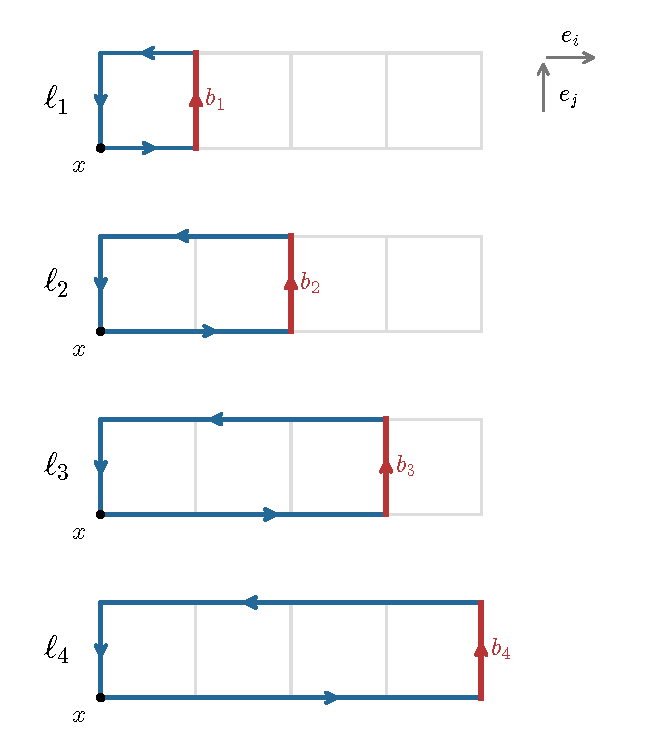
\includegraphics[width=.86\textwidth]{figures/comb_audited.pdf}
    \caption{The four loops of $\mc{C}^4_{i,j}(x)$, shown separately on
    the same strip. The loop $\ell_k$ has side lengths $k$ and $1$;
    its far short edge is used by none of the other loops. Arrows
    give the orientation in Definition \ref{def:comb}.}
    \label{fig:comb}
\end{figure}

\begin{definition}[Higgs-like field construction]\label{def:higgs-like-field}
    Fix $m$ and a nonzero intertwiner $T$ as in Lemma \ref{lm:Intertwiner-construct}. Given a gauge configuration $(Q_e)_{e\in E_{\Z^d}^+}$, define the field $(\Phi_x^{ij})_{x\in\Z^d}$ by setting
    \begin{equs}
        \Phi_x^{ij}(Q):=T\big(\sigma(Q_{\ell_1})\otimes\cdots\otimes\sigma(Q_{\ell_m})\big)\in S,
    \end{equs}
    where $(\ell_1,\dots,\ell_m)=\mc{C}^m_{i,j}(x)$ is defined in Definition \ref{def:comb}. In particular, the input to $T$ is an element of $\mc{W}_{\sigma}^{\otimes m}$.
\end{definition}
\begin{remark}[$\Phi$ in finite volume]
    We can define $\Phi_x^{ij}$ given a finite volume box gauge configuration whenever the comb $\mc{C}^m_{i,j}(x)$ is totally contained in the box.
\end{remark}

\begin{remark}[Nontriviality of $\Phi$]
    The field $\Phi_x^{ij}$ is not identically zero. Indeed, by the definition of $\mc{W}_{\sigma}$, the tensors
    \begin{equs}
        \sigma(h_1)\otimes\cdots\otimes\sigma(h_m),\qquad h_1,\ldots,h_m\in G,
    \end{equs}
    span $\mc{W}_{\sigma}^{\otimes m}$. Since $T\neq0$, there exist $h_1,\ldots,h_m\in G$ such that
    \begin{equs}
        T\big(\sigma(h_1)\otimes\cdots\otimes\sigma(h_m)\big)\neq0.
    \end{equs}
    For each $k=1,\ldots,m$, assign $Q_{b_k}=h_k$ to the edge
    \begin{equs}
        b_k=(x+ke_i,x+ke_i+e_j),
    \end{equs}
    and assign the identity to every other positively oriented edge. The loop $\ell_k$ traverses $b_k$ once in its positive orientation and none of the other $b_r$, so $Q_{\ell_k}=h_k$. Thus this gauge configuration satisfies $\Phi_x^{ij}(Q)\neq0$. The same construction works in every finite box containing the comb. \qed
\end{remark}

We now illustrate Definition \ref{def:higgs-like-field} using the intertwiner map example for $\mrm{SO}(3)$. Once again the reader only concerned with the proof of Theorem \ref{thm:Main-theorem} may skip the example.

\begin{example}[Higgs-like field for $\mrm{SO}(3)$]
    Suppose $G=\mrm{SO}(3)$, with both $\sigma$ and $\tau$ the defining representation on $\C^3$. Taking $m=1$ and $T$ from \eqref{eq:intertwiner-SO3-explicit}, the comb consists of the single plaquette $\ell_1$ based at $x$. Explicitly
    \begin{equs}
        Q_{\ell_1}=Q_{(x,x+e_i)}Q_{(x+e_i,x+e_i+e_j)}
        Q_{(x+e_j,x+e_i+e_j)}^{-1}Q_{(x,x+e_j)}^{-1}.
    \end{equs}
    Substituting $Q_{\ell_1}$ into the formula for $T$ gives
    \begin{equs}\label{eq:Phi-SO3-explicit}
        \Phi_x^{ij}(Q)=\frac16
        \begin{pmatrix}
            (Q_{\ell_1})_{23}-(Q_{\ell_1})_{32}\\
            (Q_{\ell_1})_{31}-(Q_{\ell_1})_{13}\\
            (Q_{\ell_1})_{12}-(Q_{\ell_1})_{21}
        \end{pmatrix}\in\mathbb{R}^3\subset\C^3.
    \end{equs}
    Thus the field is obtained from the antisymmetric part of the plaquette variable. Under a gauge transformation, $Q_{\ell_1}$ becomes $g_xQ_{\ell_1}g_x^{\mathsf T}$, and the equivariance of $T$ gives
    \begin{equs}
        \Phi_x^{ij}(g\cdot Q)=g_x\Phi_x^{ij}(Q).
    \end{equs}
    For a concrete nonzero value, take
    \begin{equs}
        Q_{\ell_1}=\begin{pmatrix}0&1&0\\-1&0&0\\0&0&1\end{pmatrix}\in\mrm{SO}(3).
    \end{equs}
    Then \eqref{eq:Phi-SO3-explicit} gives $\Phi_x^{ij}(Q)=e_3/3\neq0$. This plaquette variable is realized by assigning $Q_{\ell_1}$ to the edge $(x+e_i,x+e_i+e_j)$ and the identity to all other positively oriented edges. \qed
\end{example}

%\begin{example}[Higgs like field for $\mrm{SO}(2N+1)$]
%    Suppose $G=\mrm{SO}(2N+1)$ for an integer $N\geq1$, with both $\sigma$ and $\tau$ the defining representation on $\C^{2N+1}$. Take $m=N$ and $T$ from \eqref{eq:intertwiner-SOodd-explicit}. Write
    %\begin{equs}
        %(\ell_1,\ldots,\ell_N)=\mc{C}^N_{i,j}(x),
%        \qquad U_r=Q_{\ell_r},\quad r=1,\ldots,N.
%    \end{equs}
%    In particular, $U_r$ is the variable of the rectangle of side lengths $r$ and $1$ based at $x$, not the variable of its last plaquette. The field is given componentwise by
    %\begin{equs}\label{eq:Phi-SOodd-explicit}
        %\big(\Phi_x^{ij}(Q)\big)_a
        %=\frac{1}{(2N+1)!}
        %\sum_{b_1,\ldots,b_{2N}=1}^{2N+1}
        %\varepsilon_{b_1\cdots b_{2N}a}
        %\prod_{r=1}^{N}(U_r)_{b_{2r-1},b_{2r}},
   % \end{equs}
   % for $a=1,\ldots,2N+1$. Here $i,j$ are the fixed lattice directions, while the $b_r$ and $a$ are matrix indices. By antisymmetry of $\varepsilon$, replacing any $U_r$ in this formula by $(U_r-U_r^{\mathsf T})/2$ does not change its value. Thus this construction combines the antisymmetric parts of the $N$ loop variables into a vector in $\mathbb{R}^{2N+1}\subset\C^{2N+1}$. When $N=1$, the formula is exactly \eqref{eq:Phi-SO3-explicit}. Since all the loops are based at $x$, they transform simultaneously by $U_r\mapsto g_xU_rg_x^{\mathsf T}$, and the equivariance checked in the intertwiner example gives
    %\begin{equs}
        %\Phi_x^{ij}(g\cdot Q)=g_x\Phi_x^{ij}(Q).
   % \end{equs}

   % To see a nonzero value explicitly, for each $r=1,\ldots,N$ choose $U_r$ to act as
   % \begin{equs}
        %\begin{pmatrix}0&1\\-1&0\end{pmatrix}
    %\end{equs}
    %on the coordinates $(2r-1,2r)$ and as the identity on all remaining coordinates. Each $U_r$ belongs to $\mrm{SO}(2N+1)$. A nonzero summand in \eqref{eq:Phi-SOodd-explicit} must choose one of the two off-diagonal entries of each $U_r$, since diagonal entries give repeated indices in $\varepsilon$. These choices force $a=2N+1$. There are $2^N$ choices, and each contributes $1$: reversing one pair of indices changes the signs of both the matrix entry and $\varepsilon$. Consequently,
    %\begin{equs}
        %\Phi_x^{ij}(Q)=\frac{2^N}{(2N+1)!}e_{2N+1}\neq0.
   % \end{equs}
    %As in the preceding nontriviality remark, these loop variables are realized simultaneously by assigning $U_r$ to the edge $(x+re_i,x+re_i+e_j)$ for each $r$ and the identity to all other positively oriented edges. \qed
%\end{example}

%\begin{example}[Higgs like field for $\mrm{SU}(3)$ in the adjoint representation]
%    Suppose $G=\mrm{SU}(3)$, with $\sigma$ the defining representation and $\tau$ the adjoint representation on
%    \begin{equs}
        %S=\mathfrak{sl}_3(\C),\qquad \tau(g)A=gAg^*.
 %   \end{equs}
 %   Take $m=1$ and $T$ from \eqref{eq:intertwiner-SU3-explicit}. With $U=Q_{\ell_1}\in\mrm{SU}(3)$ the single plaquette variable of $\mc{C}^1_{i,j}(x)$, Definition \ref{def:higgs-like-field} becomes
    %\begin{equs}\label{eq:Phi-SU3-explicit}
        %\Phi_x^{ij}(Q)=\frac18\left(U-\frac{\mrm{Tr}U}{3}I_3\right).
   % \end{equs}
   % The matrix on the right has trace zero, so it is an element of $S$. In particular, the field is a traceless matrix viewed as a vector in the complexified adjoint space, and need not be skew-Hermitian. Under a gauge transformation, $U$ becomes $g_xUg_x^*$, so trace invariance gives
   % \begin{equs}
        %\Phi_x^{ij}(g\cdot Q)
        %&=\frac18\left(g_xUg_x^*-\frac{\mrm{Tr}U}{3}I_3\right)\\
        %&=g_x\Phi_x^{ij}(Q)g_x^*
        %=\tau(g_x)\Phi_x^{ij}(Q).
    %\end{equs}
    %For a concrete nonzero value, choose $U=\mrm{diag}(1,-1,-1)\in\mrm{SU}(3)$. Since $\mrm{Tr}U=-1$, we obtain
   % \begin{equs}
        %\Phi_x^{ij}(Q)=\frac1{12}\mrm{diag}(2,-1,-1)\neq0.
    %\end{equs}
    %As in the $\mrm{SO}(3)$ example, this plaquette variable is realized by assigning $U$ to the edge $(x+e_i,x+e_i+e_j)$ and the identity to all other positively oriented edges. \qed
%\end{example}

\begin{lemma}\label{lm:Higgs-field-transform}
    The field $\Phi_x^{ij}$ transforms like a Higgs field. More precisely, for any gauge configuration $Q$ and any gauge transformation field $g=(g_z)_{z\in\Z^d}$,
    \begin{equs}
        \Phi_x^{ij}(g\cdot Q)=\tau(g_x)\Phi_x^{ij}(Q).
    \end{equs}
    The same assertion holds in finite volume whenever the comb is contained in the box.
\end{lemma}

\begin{proof}
    For every oriented edge $e=(u,v)$ we have $(g\cdot Q)_e=g_uQ_eg_v^{-1}$. This also holds for negatively oriented edges by the convention $Q_{e^{-1}}=Q_e^{-1}$. Hence, if a path $\gamma$ has successive vertices $z_0,z_1,\ldots,z_r$, the intermediate gauge factors cancel to give
    \begin{equs}
        (g\cdot Q)_\gamma
        &=\prod_{s=1}^r\big(g_{z_{s-1}}Q_{(z_{s-1},z_s)}g_{z_s}^{-1}\big)\\
        &=g_{z_0}Q_\gamma g_{z_r}^{-1}.
    \end{equs}
    Each loop $\ell_k$ of the comb is based at $x$, so
    \begin{equs}
        \sigma\big((g\cdot Q)_{\ell_k}\big)
        =\sigma(g_x)\sigma(Q_{\ell_k})\sigma(g_x)^{-1}
        =\mrm{Ad}_\sigma(g_x)\sigma(Q_{\ell_k}).
    \end{equs}
    Applying the intertwining identity from Lemma \ref{lm:Intertwiner-construct}, we conclude that
    \begin{equs}
        \Phi_x^{ij}(g\cdot Q)
        &=T\Big(\mrm{Ad}_\sigma(g_x)^{\otimes m}
        \big(\sigma(Q_{\ell_1})\otimes\cdots\otimes\sigma(Q_{\ell_m})\big)\Big)\\
        &=\tau(g_x)T\big(\sigma(Q_{\ell_1})\otimes\cdots\otimes\sigma(Q_{\ell_m})\big)\\
        &=\tau(g_x)\Phi_x^{ij}(Q).
    \end{equs}
\end{proof}

\begin{definition}[Gluelump Wilson Line]\label{def:Wilson-Line}
    For an open path $\ell$ from points $x$ to $y$ in $\Z^d$ and gauge configuration $Q$, we define the gluelump Wilson line observable by
    \begin{equs}
        O_\ell^{ij}(Q):=\big(\Phi_x^{ij}(Q)\big)^*\tau(Q_\ell)\Phi_y^{ij}(Q),
    \end{equs}
    where $\Phi$ is defined as in Definition \ref{def:higgs-like-field}, and $\Phi^*w:=\langle\Phi,w\rangle_S$. In finite volume this observable is defined whenever the path and both endpoint combs are contained in the box.
\end{definition}

\begin{figure}[htbp]
    \centering
    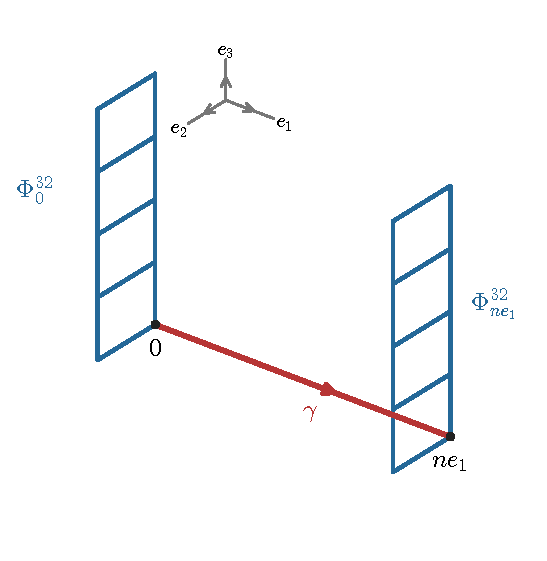
\includegraphics[width=.64\textwidth]{figures/wilson_line_audited.pdf}
    \caption{For the straight path $\gamma:0\to ne_1$ (red), the support
    of $O_{\gamma}^{32}$ also includes the blue endpoint combs, which lie in planes
    perpendicular to $e_1$. Both combs have long direction $+e_3$
    and short direction $+e_2$; $m=4$ is shown.}
    \label{fig:wilson-line}
\end{figure}


\begin{lemma}\label{lm:gluelump-gauge-invariant}
    The observable $O_\ell^{ij}$ is gauge invariant. More precisely, for every gauge configuration $Q$ and every gauge transformation field $g=(g_z)_{z\in\Z^d}$,
    \begin{equs}
        O_\ell^{ij}(g\cdot Q)=O_\ell^{ij}(Q).
    \end{equs}
    The same assertion holds in finite volume whenever the observable is defined there.
\end{lemma}

\begin{proof}
    Write $x,y$ for the initial and final vertices of $\ell$. The path calculation in the preceding proof gives
    \begin{equs}
        \tau\big((g\cdot Q)_\ell\big)
        =\tau(g_x)\tau(Q_\ell)\tau(g_y)^{-1}.
    \end{equs}
    Using Lemma \ref{lm:Higgs-field-transform} at both endpoints and the unitarity of $\tau$, we obtain
    \begin{equs}
        O_\ell^{ij}(g\cdot Q)
        &=\big(\tau(g_x)\Phi_x^{ij}(Q)\big)^*
        \tau(g_x)\tau(Q_\ell)\tau(g_y)^{-1}
        \tau(g_y)\Phi_y^{ij}(Q)\\
        &=\big(\Phi_x^{ij}(Q)\big)^*
        \tau(g_x)^*\tau(g_x)\tau(Q_\ell)\Phi_y^{ij}(Q)\\
        &=\big(\Phi_x^{ij}(Q)\big)^*\tau(Q_\ell)\Phi_y^{ij}(Q)
        =O_\ell^{ij}(Q).
    \end{equs}
\end{proof}
\subsection{Reflection positivity argument}\label{sec:reflection-argument}

In the last section we constructed a nonzero field assigned to vertices which transforms like a Higgs field under gauge transformations.
In this section we use arguments based on reflection positivity which first appeared in the Yang--Mills--Higgs case \cite{EvertzEtAl1987Perimeter} to complete the proof of Theorem \ref{thm:Main-theorem}.

The first step is to bound the expectation of the one-edge Wilson line $O_e^{ij}$ below by a positive constant independent of the volume. We begin with a standard gauge-fixing procedure.

\begin{lemma}[Gauge fixing to identity on a forest]
\label{lm:gauge-fix-to-identity}
Let $\Lambda\subset\Z^d$ be a finite subgraph, and let
$F\subset E_\Lambda^+$ be a set of edges whose underlying unoriented
graph contains no cycles. For
$R\in G^{E_\Lambda^+\setminus F}$, define the gauge configuration
$R^F$ by
\begin{equs}
    R_e^F:=
    \begin{cases}
        \groupid,&e\in F,\\
        R_e,&e\in E_\Lambda^+\setminus F.
    \end{cases}
\end{equs}
For every bounded Borel gauge-invariant function $h$,
\begin{equs}\label{eq:forest-gauge-fixing}
    \int_{G^{E_\Lambda^+}}h(R)\,dR
    =
    \int_{G^{E_\Lambda^+\setminus F}}h(R^F)\,dR.
\end{equs}
Here each integral uses product normalized Haar measure on the indicated edge set. Consequently, writing $S=S_{G,\sigma,\Lambda,\beta}$, every bounded
Borel gauge-invariant observable $f$ satisfies
\begin{equs}\label{eq:forest-gauge-fixing-ym}
    \langle f\rangle_\Lambda
    =
    \frac{\displaystyle
        \int_{G^{E_\Lambda^+\setminus F}}
        f(R^F)e^{S(R^F)}\,dR}
    {\displaystyle
        \int_{G^{E_\Lambda^+\setminus F}}
        e^{S(R^F)}\,dR}.
\end{equs}
\end{lemma}

We defer the proof to Appendix \ref{sec:Gauge-fix} as the lemma is well known. 

We are now ready to state and prove the lower bound on $O_e^{ij}$.
\begin{lemma}[One-edge positivity]\label{lm:one-edge-positivity}
    For $d \geq 3$ and any $\beta>0$, there exists a constant $c=c(d,\beta,G,\sigma,\tau)>0$ such that if $e \in E_{\Z^d}$ and $i,j$ are distinct coordinate directions perpendicular to $e$,
    \begin{equs}
        \langle O_e^{ij}\rangle>c.
    \end{equs}
    The constant may depend on the fixed choice of $m,T$ in the definition of $\Phi_x^{ij}$; these are chosen once for $G,\sigma,\tau$.
\end{lemma}

\begin{proof}
First work in $\Lambda_L^k$ with $e=(0,e_k)$ and distinct
$i,j\neq k$, taking $L$ large enough to contain both endpoint combs.
By Lemmas \ref{lm:gluelump-gauge-invariant} and
\ref{lm:gauge-fix-to-identity}, we may fix all edges crossing
$\{x_k=1/2\}$ to $\groupid$, since they form a forest.
Identify the two half-boxes by reflection with
$H_L^k:=\Lambda_L^k\cap\{x:x_k\leq0\}$, and write their
configurations as $Q,Q'$ and their product Haar measures as $dQ,dQ'$.
Then $O_e^{ij}=\Phi(Q)^*\Phi(Q')$, where $\Phi=\Phi_0^{ij}$.

Let $J$ be the set of $3m+1$ positively oriented edges in
$\mc{C}^m_{i,j}(0)$. Each unoriented plaquette crossing
$\{x_k=1/2\}$ contributes
$2\beta\mrm{Re}\,\mrm{Tr}(\sigma(Q_b)\sigma(Q'_b)^*)$
to the action, where $b$ is its positively oriented edge in
$\{x_k=0\}$. Remove just the crossing-plaquette factors indexed by
$b\in J$, and denote the remaining weight by
\begin{equs}
    w(Q,Q')
    &:=\exp\big(S_{G,\sigma,H_L^k,\beta}(Q)
               +S_{G,\sigma,H_L^k,\beta}(Q')\big)\\
    &\quad\times
    \prod_{\substack{b\in E_{H_L^k}^+\setminus J\\
                     b\subset\{x_k=0\}}}
    \exp\big(2\beta\mrm{Re}\,\mrm{Tr}
                 (\sigma(Q_b)\sigma(Q'_b)^*)\big).
\end{equs}
Expanding only the crossing-plaquette factors gives
\begin{equs}
    w(Q,Q')=\sum_\nu f_\nu(Q)\overline{f_\nu(Q')},
\end{equs}
where $\nu$ ranges over a countable index set and each $f_\nu$ is a
nonnegative constant times $e^{S_{G,\sigma,H_L^k,\beta}(Q)}$
times a monomial in the entries of the remaining boundary-edge
matrices $\sigma(Q_b)$ and their conjugates.

In an orthonormal basis of $V$, let $p_\alpha$ be the monomial
with multi-index $\alpha$ in the entries of
$(\sigma(Q_b))_{b\in J}$ and their conjugates, and write
$\alpha!=\prod_s\alpha_s!$.
The deleted factors expand as 
\begin{equs}
    \prod_{b \in J}\exp(2\beta \mrm{Re}\mrm{Tr}(\sigma(Q_b)\sigma(Q_b')^*))=\sum_{\alpha} \frac{\beta^{|\alpha|}}{\alpha!}p_{\alpha}(Q)\overline{p_{\alpha}(Q')}.
\end{equs}
All these series converge absolutely and uniformly for each fixed $L$.

Each rectangle $\ell_k$ has $2k+2$ edge occurrences, so
$\Phi$ has a homogeneous polynomial expansion
\begin{equs}
 \Phi=\sum_{|\alpha|=D}v_\alpha p_\alpha,\qquad \text{with } \hspace{2mm}
 D:=\sum_{k=1}^m(2k+2)=m(m+3).
\end{equs}
Here $v_\alpha\in S$, and $D$ counts occurrences with repetitions, not the $3m+1$ distinct
comb edges. Each comb edge corresponds to one unoriented crossing
plaquette, but its Taylor expansion may supply several factors.
Thus a monomial of degree $D$ carries the coefficient
$\beta^D/\alpha!$ in the crossing-kernel expansion.
The unnormalized numerator is therefore
\begin{equs}
    \sum_{\nu,\alpha}\frac{\beta^{|\alpha|}}{\alpha!}
    \left\|\int\Phi\,\overline{p_\alpha f_\nu}\,dQ\right\|^2.
\end{equs}
For every $\nu$, weighted Cauchy--Schwarz gives
\begin{equs}
 \left|\int\|\Phi\|^2\overline{f_\nu}\,dQ\right|^2
 &=\left|\sum_{|\alpha|=D}v_\alpha^*
       \int\Phi\,\overline{p_\alpha f_\nu}\,dQ\right|^2\\
 &\leq C_\Phi\sum_{|\alpha|=D}\frac1{\alpha!}
       \left\|\int\Phi\,\overline{p_\alpha f_\nu}\,dQ\right\|^2,
\end{equs}
where $C_\Phi:=\sum_{|\alpha|=D}\alpha!\|v_\alpha\|^2>0$ since $\Phi$ is nonzero.

Consequently, retaining only terms with $|\alpha|=D$, the numerator is at least
\begin{equs}
 \frac{\beta^D}{C_\Phi}
 \sum_\nu\left|\int\|\Phi\|^2\overline{f_\nu}\,dQ\right|^2
 =\frac{\beta^D}{C_\Phi}
 \iint\|\Phi(Q)\|^2\|\Phi(Q')\|^2
                 w(Q,Q')\,dQ\,dQ'.
\end{equs}
The equality above follows from Fubini and the definition of $w(Q,Q')$.

Under the probability measure proportional to $w\,dQ\,dQ'$,
condition on all edges outside $J$ in both halves.
Each comb edge meets at most $2(d-2)+1=2d-3$ half-box plaquettes.
Thus at most $2(2d-3)|J|$ unoriented plaquettes depend on the remaining
variables, each with action oscillation at most $4\beta n$ for
$n:=\mrm{dim}\,V$.
Their conditional density relative to product Haar measure is
therefore at least $e^{-8\beta n(2d-3)|J|}$.
Moreover, $a:=\int_{G^J}\|\Phi\|^2dQ>0$: by nontriviality and
continuity, $\|\Phi\|^2$ is bounded below by a positive constant
on a fixed nonempty open set, which has positive Haar measure.
The normalizing denominator is at most
$e^{2\beta n|J|}\iint w\,dQ\,dQ'$. Consequently,
\begin{equs}
 \langle O_e^{ij}\rangle_{\Lambda_L^k}
 \geq \frac{a^2\beta^D}{C_\Phi}
 e^{-2\beta n(8d-11)(3m+1)}.
\end{equs}
This bound is independent of $L$. Pass to the limit by
Assumption \ref{as:infinite-vol}, since $O_e^{ij}$ is bounded,
continuous and local. Translation invariance and
$O_{e^{-1}}^{ij}=\overline{O_e^{ij}}$ give the bound for every oriented edge.
\end{proof}

\begin{remark}[Dependence of the constant]
Fix $m,T$ and the polynomial expansion above, independently of
$\beta,L$. One may take
\begin{equs}
 c=\frac{a^2}{2C_\Phi}\,
 \beta^{m(m+3)}
 \exp\{-2\beta(\mrm{dim}\,V)(8d-11)(3m+1)\}.
\end{equs}
The factor $1/2$ gives the strict inequality in the lemma.
Integrating first the $m$ edges $(re_i,re_i+e_j)$,
$1\leq r\leq m$, gives
\begin{equs}
 a=\int_{G^m}
 \left\|T\big(\sigma(Q_1)\otimes\cdots\otimes\sigma(Q_m)\big)\right\|^2
 \,dQ_1\cdots dQ_m>0.
\end{equs}
Thus $a$ and the explicit coefficient sum $C_\Phi$ depend only
on $G,\sigma$ and the fixed choice of $m,T$, not on the volume,
$\beta$ or $d$. 
\end{remark}

We now record the three forms of reflection positivity used below.
For a lattice reflection hyperplane $P$, let $\Theta_P$ denote reflection
of vertices, and set
\begin{equs}
    \Theta_P(x,y)&:=(\Theta_Px,\Theta_Py),\\
    (\Theta_PQ)_e&:=Q_{\Theta_Pe},\qquad
    (\Theta_Pf)(Q):=f(\Theta_PQ).
\end{equs}
We first work in a finite subgraph $\Lambda$ invariant under $\Theta_P$.
All functions below are continuous and take values in a finite-dimensional
complex Hilbert space $\mathcal K$, with inner product conjugate-linear
in the first argument. Support in a half space means that every edge
on which the function depends has both endpoints in that half space;
edges contained in $P$ are allowed. For site and diagonal reflections,
write
\begin{equs}
    B_P(f,g):=\big\langle\langle f,\Theta_Pg\rangle_{\mathcal K}
        \big\rangle_\Lambda.
\end{equs}
For bond reflections, the corresponding pairing uses the gauge invariant
gluing specified below.

\begin{lemma}[Site Reflection Positivity]\label{lm:site-reflection-positivity}
Let $P=\{x:x_k=a\}$, where $k\in\{1,\ldots,d\}$ and $a\in\Z$.
Let $f,g$ be $\mathcal K$-valued functions supported in
$\Lambda\cap\{x:x_k\geq a\}$. Then
$B_P(f,g)=\overline{B_P(g,f)}$, and
\begin{equs}\label{eq:site-RP-CS}
    B_P(f,f),\ B_P(g,g)&\geq0,\\
    |B_P(f,g)|^2&\leq B_P(f,f)B_P(g,g).
\end{equs}
\end{lemma}

\begin{lemma}[Bond Reflection Positivity]\label{lm:bond-reflection-positivity}
Let $P=\{x:x_k=a+\tfrac12\}$, where $k\in\{1,\ldots,d\}$ and $a\in\Z$.
Let $f,g$ be $\mathcal K$-valued functions supported in
$\Lambda\cap\{x:x_k\geq a+1\}$. Suppose that, for
$h,h'\in\{f,g\}$, there are continuous gauge-invariant scalar observables
$A_{h,h'}$ satisfying
\begin{equs}\label{eq:bond-RP-gluing}
    A_{h,h'}(Q)=\langle h(Q),\Theta_Ph'(Q)\rangle_{\mathcal K}
    \quad\text{whenever every edge crossing $P$ has variable $\groupid$.}
\end{equs}
In this case, set $B_P(h,h'):=\langle A_{h,h'}\rangle_\Lambda$.
Then $B_P(f,g)=\overline{B_P(g,f)}$, and
\begin{equs}\label{eq:bond-RP-CS}
    B_P(f,f),\ B_P(g,g)&\geq0,\\
    |B_P(f,g)|^2&\leq B_P(f,f)B_P(g,g).
\end{equs}
\end{lemma}

\begin{lemma}[Diagonal Reflection Positivity]\label{lm:diagonal-reflection-positivity}
Let $P=\{x:x_k-sx_l=a\}$, where $k,l\in\{1,\ldots,d\}$ are distinct,
$s\in\{-1,1\}$ and $a\in\Z$.
Let $f,g$ be $\mathcal K$-valued functions supported in
$\Lambda\cap\{x:x_k-sx_l\geq a\}$. Then
$B_P(f,g)=\overline{B_P(g,f)}$, and
\begin{equs}\label{eq:diagonal-RP-CS}
    B_P(f,f),\ B_P(g,g)&\geq0,\\
    |B_P(f,g)|^2&\leq B_P(f,f)B_P(g,g).
\end{equs}
\end{lemma}

% Citation checked against SO3_deconfinement_reflection_positivity_updated.tex
% (13 October 2026), subsection:Ref-Pos, lemma lm:reflec-pos and its proof.
% The subsection and lemma title identify the revised argument without
% retaining the superseded arXiv page and lemma numbers.
For the coordinate reflection argument, including the gauge invariant
gluing formulation for bond reflections, see the ``Reflection positivity''
lemma and its proof in
\cite[Subsection~3.3]{nissim2026deconfinementmathrmso3latticeyangmills}.
For the present compact group and Wilson action, the same finite-volume
proof uses the positive crossing-kernel expansion from
Lemma \ref{lm:one-edge-positivity}; its Hilbert-space-valued form follows
by applying the scalar argument to each coordinate.
For the diagonal reflection argument, see
\cite[pp.~278--279, equations~(9)--(13)]{EvertzEtAl1987Perimeter};
the Hilbert-space-valued version follows by summing the scalar
pairings over an orthonormal basis and applying Cauchy--Schwarz.

Under Assumption \ref{as:infinite-vol}, all three statements also hold
for continuous local functions in infinite volume, with
$\langle\cdot\rangle_\Lambda$ replaced by $\langle\cdot\rangle$ in the
definition of $B_P$. Indeed, for the site plane $x_k=0$ use
$\Lambda_L^j$ with $j\neq k$; for the bond plane $x_k=1/2$ use
$\Lambda_L^k$; and for the diagonal plane $x_k-sx_l=0$ use
$\Lambda_L^j$ with $j\notin\{k,l\}$. These boxes are reflection
invariant, and the last choice is possible because $d\geq3$.
The finite-volume inequalities pass to the limit by weak convergence.
Integer translations give the other planes, and reflection invariance
gives the statements for either half space. We use this infinite-volume
pairing $B_P$ from now on.

\begin{remark}[Wilson loops and Wilson lines]\label{rem:RP-Wilson-observables}
For a bond plane $P=\{x:x_k=a+\tfrac12\}$, write
$b_v=(v,\Theta_Pv)$ when $v_k=a+1$.
For paths $\gamma,\eta$ from the same boundary vertex $v$ to the same
boundary vertex $w$, both in $\{x:x_k\geq a+1\}$, take
$f=\tau(Q_\gamma)$ and $g=\tau(Q_\eta)$ with the normalized
Hilbert--Schmidt inner product
$\langle A,B\rangle=(\dim\tau)^{-1}\mrm{Tr}(A^*B)$. Their gluing is
\begin{equs}\label{eq:RP-loop-gluing}
    A_{f,g}
    &=\frac1{\dim\tau}\mrm{Tr}\big(
        f^*\tau(Q_{b_v})(\Theta_Pg)\tau(Q_{b_w})^*\big)\\
    &=W^\tau_{\gamma^{-1}b_v(\Theta_P\eta)b_w^{-1}}.
\end{equs}
For paths $\gamma:v\to x$ and $\eta:v\to y$ whose paths and endpoint
combs lie in the same half space, instead take
\begin{equs}
    f=\tau(Q_\gamma)\Phi_x^{ij},\qquad
    g=\tau(Q_\eta)\Phi_y^{ij},\qquad
    A_{f,g}=f^*\tau(Q_{b_v})\Theta_Pg.
\end{equs}
In both cases, the other pairings are defined in the same way.
The gauge factors cancel in each $A_{h,h'}$, and setting the crossing
edge variables to $\groupid$ gives \eqref{eq:bond-RP-gluing}.
Thus it is the glued observable, not each half-observable, that must
be gauge invariant.
For site and diagonal reflections the cut vertices lie in $P$, and
the crossing-edge factors are omitted. Always reflect the entire
ordered endpoint comb: for a bond reflection with $i,j\neq k$,
$\Theta_P\Phi_x^{ij}=\Phi_{\Theta_Px}^{ij}$, whereas a diagonal
reflection may change its directions.
\end{remark}

We now propagate the one-edge lower bound through straight paths,
L-shaped paths and squares. Coordinate reflections then compare
arbitrary rectangles with squares; see Figures \ref{fig:reflection-L} and \ref{fig:reflection-square}.

\begin{proof}[Proof of Theorem \ref{thm:Main-theorem}]
Fix the coordinate plane of the rectangle, label its directions $1,2$,
and choose a third direction $3$. Normalize $T$ so that
$\|\Phi_x^{ij}(Q)\|\leq1$ for every $x,i,j,Q$, and fix
$0<c<1$ supplied by Lemma \ref{lm:one-edge-positivity} for this
normalization. For integers $r,s\geq0$, write
$w_{r,s}:=\langle W_{\ell_{r,s}}^\tau\rangle$, where
$\ell_{r,s}$ follows the coordinate paths through
$0,re_1,re_1+se_2,se_2,0$. In particular,
$w_{0,s}=w_{r,0}=1$ by backtracking.

\emph{From one edge to a straight path.}
For $n\geq0$, let $\gamma_n$ be the straight path from $0$ to $ne_1$,
with $\gamma_0$ the empty path, and set
\begin{equs}
    g_n:=\langle O_{\gamma_n}^{32}\rangle.
\end{equs}
For integers $r,s\geq0$, apply site and bond reflection positivity to
\begin{equs}
    f=\tau(Q_{\gamma_r})\Phi_{re_1}^{32},\qquad
    g=\tau(Q_{\gamma_s})\Phi_{se_1}^{32},
\end{equs}
with planes $\{z:z_1=0\}$ and $\{z:z_1=-1/2\}$, respectively.
The combs are transverse to direction $1$. Gluing the two half-paths
gives a reversed straight path of length $r+s$ in the site case and
$r+s+1$ in the bond case. The bond gluing is the gauge invariant
Wilson line described in Remark \ref{rem:RP-Wilson-observables}.
By translation invariance and path reversal, the two pairings are
$\overline{g_{r+s}}$ and $\overline{g_{r+s+1}}$. Taking $f=g$ first
shows that every $g_n$ is real and nonnegative; for general $r,s$,
Cauchy--Schwarz gives
\begin{equs}
    g_{r+s}^2&\leq g_{2r}g_{2s},\\
    g_{r+s+1}^2&\leq g_{2r+1}g_{2s+1}.
\end{equs}
Taking $s=r+1$ gives, respectively, the odd and even cases of
\begin{equs}
    g_n^2\leq g_{n-1}g_{n+1},\qquad n\geq1.
\end{equs}
Since $g_1>c$, these inequalities imply that every $g_n>0$ and that
$g_n/g_{n-1}$ is nondecreasing. Also
$g_0=\langle\|\Phi_0^{32}\|^2\rangle\leq1$, so
\begin{equs}\label{eq:main-straight-lower-bound}
    g_n\geq\frac{g_1^n}{g_0^{n-1}}\geq c^n,\qquad n\geq1.
\end{equs}

\emph{From a straight path to an L shape.}
Fix $n\geq1$, put $x=ne_1$, $y=ne_2$, and let $\lambda_n$ be the
path $x\to0\to y$. For $P=\{z:z_1=z_2\}$, take
\begin{equs}
    f=\tau(Q_{\gamma_n})\Phi_x^{32},\qquad g=\Phi_0^{31}.
\end{equs}
Both are supported in $\{z:z_1\geq z_2\}$: the comb at $x$ has
$z_1=n$ and $0\leq z_2\leq1$, while the comb at $0$ has
$z_2=0$ and $0\leq z_1\leq1$. Reflection interchanges directions
$1,2$ and preserves the ordering of the combs, so
$\Theta_P\Phi_x^{32}=\Phi_y^{31}$ and
$\Theta_P\Phi_0^{31}=\Phi_0^{32}$. Hence
\begin{equs}
    B_P(f,g)&=\overline{g_n}=g_n,\\
    B_P(f,f)&=\big\langle(\Phi_x^{32})^*
        \tau(Q_{\lambda_n})\Phi_y^{31}\big\rangle,\\
    0&\leq B_P(g,g)\leq1.
\end{equs}
The last bound follows from reflection positivity and the pointwise
norm bound on $\Phi$. Therefore diagonal Cauchy--Schwarz gives
\begin{equs}
    \big\langle(\Phi_x^{32})^*
        \tau(Q_{\lambda_n})\Phi_y^{31}\big\rangle
    \geq g_n^2\geq c^{2n}.
\end{equs}

\emph{From an L shape to a square.}
Now take $P=\{z:z_1+z_2=n\}$ and, with the unnormalized
Hilbert--Schmidt inner product on $\mrm{End}_{\C}(S)$, set
\begin{equs}
    f=\tau(Q_{\lambda_n}),\qquad
    g=\Theta_P\big(\Phi_x^{32}(\Phi_y^{31})^*\big).
\end{equs}
The path $\lambda_n$ lies in $\{z:z_1+z_2\leq n\}$, whereas the
original endpoint combs lie in $\{z:z_1+z_2\geq n\}$.
Indeed, their vertices have the forms $(n,u,t)$ and $(u,n,t)$,
with $u\in\{0,1\}$ and $t\in\{0,\ldots,m\}$ (other coordinates
are zero). Reflection sends these vertices to $(n-u,0,t)$ and
$(0,n-u,t)$, respectively. Thus both $f$ and the reflected product
$g$ are supported in $\{z:z_1+z_2\leq n\}$. Reflection fixes $x,y$ and
sends $0$ to $n(e_1+e_2)$, so
\begin{equs}
    B_P(f,f)&=(\dim\tau)w_{n,n},\\
    B_P(f,g)&=\overline{\big\langle(\Phi_x^{32})^*
        \tau(Q_{\lambda_n})\Phi_y^{31}\big\rangle},\\
    0&\leq B_P(g,g)\leq1.
\end{equs}
The first identity glues $\lambda_n^{-1}$ to its reflection to form
the square; the second follows from cyclicity of the trace; and the
last uses $\|g\|_{\mrm{HS}},\|\Theta_Pg\|_{\mrm{HS}}\leq1$.
Another Cauchy--Schwarz inequality yields
\begin{equs}\label{eq:main-square-lower-bound}
    w_{n,n}
    &\geq\frac1{\dim\tau}
        \left|\big\langle(\Phi_x^{32})^*
        \tau(Q_{\lambda_n})\Phi_y^{31}\big\rangle\right|^2\\
    &\geq\frac{c^{4n}}{\dim\tau}.
\end{equs}

\emph{From squares to rectangles.}
For fixed $s$, apply site and bond reflection positivity to the
matrix-valued holonomies of the two paths
\begin{equs}
    0\to ae_1\to ae_1+se_2\to se_2,\qquad
    0\to be_1\to be_1+se_2\to se_2,
\end{equs}
where $a,b\geq0$, using the same planes as in the straight-path step
and the normalized Hilbert--Schmidt inner product. The gauge invariant
gluings of Remark \ref{rem:RP-Wilson-observables} give rectangles of
widths $a+b$ and $a+b+1$, respectively. Taking equal half-paths and
then consecutive widths, just as above, gives
\begin{equs}
    0\leq w_{r,s}\leq1,\qquad
    w_{r,s}^2\leq w_{r-1,s}w_{r+1,s}\quad(r\geq1),
\end{equs}
where the upper bound follows from unitarity. The same argument
applies in $s$. These inequalities imply that $w_{r,s}$ is
nonincreasing in each variable. Indeed, an increasing step would
force both terms to be positive by log-convexity, and subsequent
ratios would remain bounded below by a number greater than one,
contradicting $w_{r,s}\leq1$.
Taking $n=\max\{r,s\}$ in \eqref{eq:main-square-lower-bound}, we obtain,
for $r,s\geq1$,
\begin{equs}
    w_{r,s}&\geq w_{n,n}\geq\frac{c^{4\max\{r,s\}}}{\dim\tau}
        \geq\exp\{-C_\beta|\ell_{r,s}|\},\\
    C_\beta&:=2\log\frac1c+\frac14\log(\dim\tau),
\end{equs}
since $|\ell_{r,s}|=2(r+s)\geq4$.
Translation invariance gives every coordinate rectangle; reversing
its orientation conjugates its already real expectation. The
quantitative bound on $c$ from Lemma \ref{lm:one-edge-positivity}
gives $C_\beta\leq C_{G,\sigma,\tau,d}(1+\beta+|\log\beta|)$,
as detailed in the following remark.
\end{proof}

\begin{figure}[htbp]
    \centering
    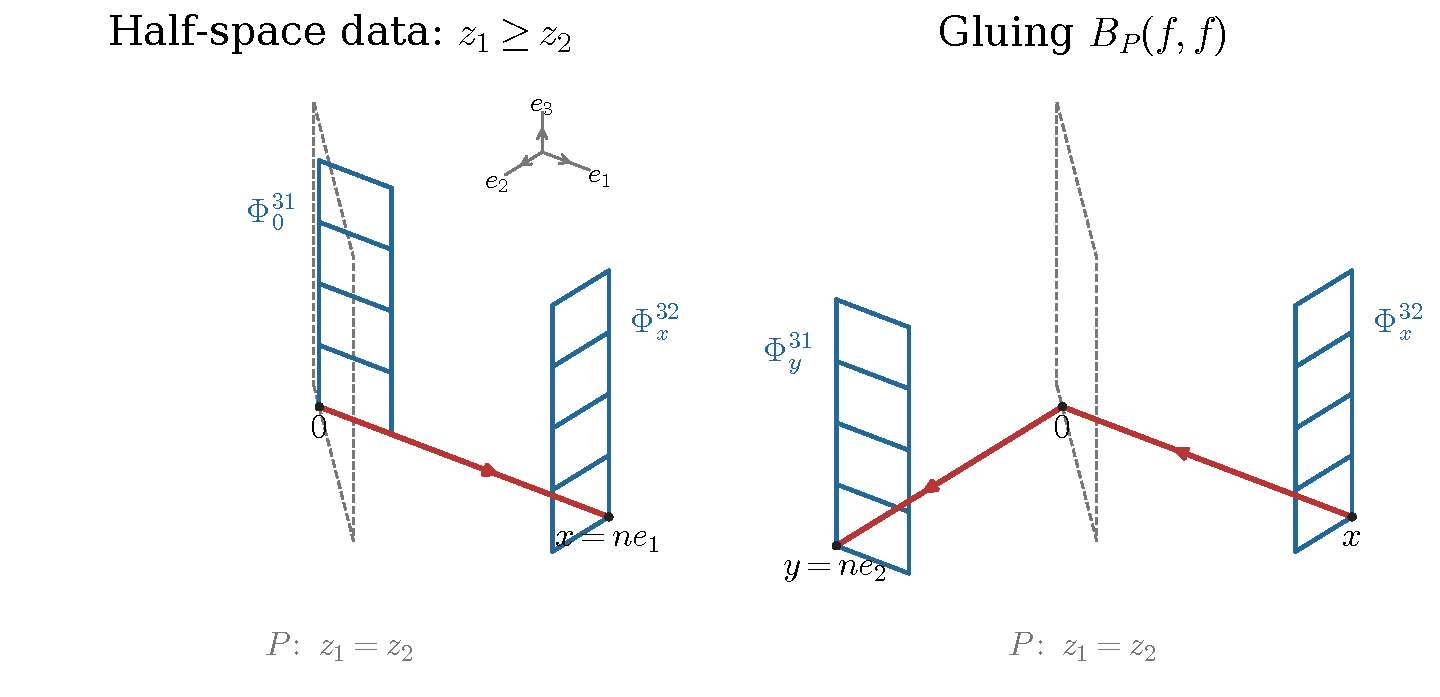
\includegraphics[width=\textwidth]{figures/reflection_L_audited.pdf}
    \caption{Reflection in $P=\{z_1=z_2\}$, shown by the dashed frame.
    Left: the red path and blue combs support
    $f=\tau(Q_{\gamma_n})\Phi_x^{32}$ and $g=\Phi_0^{31}$,
    entirely in $\{z_1\geq z_2\}$.
    Right: the gluing $B_P(f,f)$ gives the L-shaped path
    $x\to0\to y$, with endpoint fields $\Phi_x^{32}$ and
    $\Phi_y^{31}$. Here $x=ne_1$, $y=ne_2$ and $m=4$;
    all combs have long direction $+e_3$.}
    \label{fig:reflection-L}
\end{figure}

\begin{figure}[htbp]
    \centering
    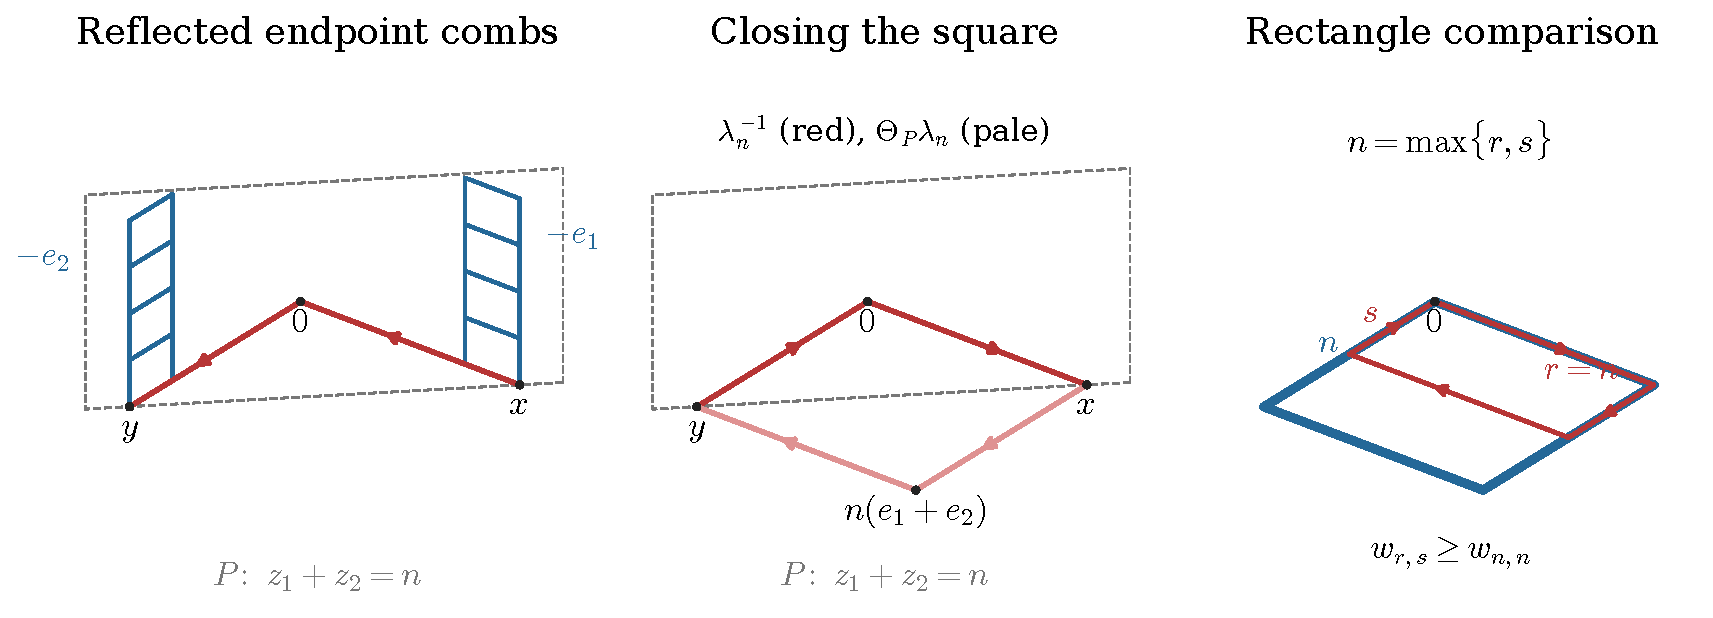
\includegraphics[width=\textwidth]{figures/reflection_square_audited.pdf}
    \caption{Left: for $P=\{z_1+z_2=n\}$, the red L-shaped path
    supports $f=\tau(Q_{\lambda_n})$ and the blue combs support
    $g=\Theta_P(\Phi_x^{32}(\Phi_y^{31})^*)$.
    Both supports lie in $\{z_1+z_2\leq n\}$; the blue combs
    are reflected combs, with short directions $-e_1$ at $x$
    and $-e_2$ at $y$.
    Middle: $\lambda_n^{-1}$ (red) and $\Theta_P\lambda_n$
    (pale red) form the square in $B_P(f,f)$.
    Right: the red $r\times s$ rectangle lies in the blue
    $n\times n$ square, $n=\max\{r,s\}$, illustrating the
    comparison $w_{r,s}\geq w_{n,n}$, not another diagonal reflection.}
    \label{fig:reflection-square}
\end{figure}

\begin{remark}[Quantitative dependence on $\beta$]
For the fixed normalized choice of $T$, retain $a,C_\Phi$ from the
remark following Lemma \ref{lm:one-edge-positivity}. Set
\begin{equs}
    D=m(m+3),\qquad
    K=2(\mrm{dim}\,V)(8d-11)(3m+1).
\end{equs}
That lemma permits the choice
\begin{equs}
    c&=\frac{a^2}{2C_\Phi}\beta^D e^{-K\beta},\\
    C_\beta&=2K\beta+2D\log\frac1\beta
        +2\log\frac{2C_\Phi}{a^2}
        +\frac14\log(\mrm{dim}\,\tau).
\end{equs}
In particular, for some $C_{G,\sigma,\tau,d}$ independent of
$\beta$, the volume, and the rectangle,
\begin{equs}
    \langle W_\ell^\tau\rangle
    \geq\exp\big\{-C_{G,\sigma,\tau,d}
        (1+\beta+|\log\beta|)|\ell|\big\},\qquad\beta>0.
\end{equs}
The displayed choice of $C_\beta$ is
$2m(m+3)|\log\beta|+O_{G,\sigma,\tau,d}(1)$ as
$\beta\downarrow0$, and is $O_{G,\sigma,\tau,d}(\beta)$ as
$\beta\to\infty$. The linear term in $\beta$ comes from the local
conditional-density comparison in Lemma \ref{lm:one-edge-positivity};
the present argument does not give an $O(\log\beta)$ perimeter
rate as $\beta\to\infty$.
\end{remark}


\appendix
\section{An elementary Haar integral}\label{Appendix:Expectation-Values}

\begin{proof}[Proof of Lemma \ref{lm:odd-SO-determinant-moment}]
    For $i_1,\ldots,i_n\in\{1,\ldots,n\}$, write
    \begin{equs}
        I(i_1,\ldots,i_n):=\int_{\mrm{SO}(n)}Q_{i_1 1}\cdots Q_{i_n n}\,dQ,
    \end{equs}
    and let $r_a$ be the number of occurrences of $a$ among $i_1,\ldots,i_n$.
    Fix distinct $a,b\in\{1,\ldots,n\}$, and let $D_{ab}$ be the diagonal matrix whose entries in positions $a,b$ are $-1$ and whose other diagonal entries are $1$. Since $D_{ab}\in\mrm{SO}(n)$, left invariance of Haar measure gives
    \begin{equs}
        I(i_1,\ldots,i_n)=(-1)^{r_a+r_b}I(i_1,\ldots,i_n).
    \end{equs}
    Consequently, a nonzero integral requires $r_a+r_b$ to be even for every $a\neq b$, so all the $r_a$ have the same parity. Since $\sum_{a=1}^n r_a=n$ is odd, they cannot all be even. They must therefore all be odd, and hence all equal to $1$. In particular, the integral vanishes whenever two indices coincide.

    Now suppose the indices are distinct. Fix distinct row labels $a,b$, and let $R_{ab}\in\mrm{SO}(n)$ act on rows by
    \begin{equs}
        (R_{ab}Q)_{a k}=Q_{b k},\qquad
        (R_{ab}Q)_{b k}=-Q_{a k},\qquad
        (R_{ab}Q)_{c k}=Q_{c k}\quad(c\notin\{a,b\}).
    \end{equs}
    The tuple $(i_1,\ldots,i_n)$ contains each of $a,b$ exactly once. Thus the substitution $Q\mapsto R_{ab}Q$ shows that interchanging the labels $a,b$ in this tuple changes the sign of the integral. Every permutation is a product of transpositions, so
    \begin{equs}
        I(i_1,\ldots,i_n)=c\varepsilon_{i_1\cdots i_n},
        \qquad c:=I(1,\ldots,n).
    \end{equs}
    Finally, let $\mrm{S}_n$ denote the permutation group on $\{1,\ldots,n\}$. Expanding $\det Q=1$ and integrating, we find
    \begin{equs}
        1
        &=\int_{\mrm{SO}(n)}\det Q\,dQ\\
        &=\sum_{\pi\in\mrm{S}_n}\mrm{sgn}(\pi)
        I\big(\pi(1),\ldots,\pi(n)\big)\\
        &=\sum_{\pi\in\mrm{S}_n}\mrm{sgn}(\pi)^2c
        =n!c.
    \end{equs}
    Hence $c=1/n!$, as claimed.
\end{proof}

\section{Gauge fixing along a forest}\label{sec:Gauge-fix}

\begin{proof}[Proof of Lemma \ref{lm:gauge-fix-to-identity}]
Choose a root in each connected component of the forest with vertex
set $\Lambda$ and edge set $F$, including its isolated vertices.
Fix the forest variables $q=(q_e)_{e\in F}$. For each vertex $v$,
let $\gamma_v$ be the unique path in the forest from its root to $v$,
and set
\begin{equs}
    \phi_v:=q_{\gamma_v},
\end{equs}
with the empty product equal to $\groupid$ and reversed edges
assigned inverse group elements. These gauge factors depend only
on $q$. If $y$ is a child of $x$ in a rooted tree, then
$\phi_y=\phi_xq_{(x,y)}$. Thus the gauge transformation
$\mc{G}_q$ specified by $(\phi_v)_{v\in\Lambda}$ sends every forest
edge to $\groupid$, in either orientation.

Keep $Q_e=q_e$ for $e\in F$.
For fixed $q$, the remaining transformed variables are
\begin{equs}
    R_e=\phi_xQ_e\phi_y^{-1},
    \qquad e=(x,y)\in E_\Lambda^+\setminus F.
\end{equs}
This is a bijective change of variables preserving product Haar
measure, since each $\phi_v$ is now fixed and Haar measure is
left and right invariant. Moreover,
$\mc{G}_qQ=R^F$. Gauge invariance of $h$ and Fubini's theorem
therefore give
\begin{equs}
    \int h(Q)\,dQ
    &=\int_{G^F}\int_{G^{E_\Lambda^+\setminus F}}
        h\big(\mc{G}_qQ\big)\,dQ\,dq\\
    &=\int_{G^F}\int_{G^{E_\Lambda^+\setminus F}}
        h(R^F)\,dR\,dq\\
    &=\int_{G^{E_\Lambda^+\setminus F}}h(R^F)\,dR.
\end{equs}
The last equality uses $\int_{G^F}dq=1$. This proves
\eqref{eq:forest-gauge-fixing}. Under a gauge transformation,
each plaquette holonomy is conjugated at its basepoint, so its
character, and hence $S$, is unchanged. Applying
\eqref{eq:forest-gauge-fixing} to $h=fe^S$ and to $h=e^S$ proves
\eqref{eq:forest-gauge-fixing-ym}.
\end{proof}


\bibliographystyle{alpha}
%\bibliographystyle{plainnat}
\bibliography{references}

\end{document}
